The present chapter describes the theoretical frame needed to understand and motivate the physical contents of this thesis. 
It firstly introduces the Standard Model of particle physics, a theory that describes the foundations that rule the subatomic world. 

%++++++++++++++++++++++++++++++++++++++++++++++
\section{The Standard Model of Particle Physics}
\label{sec:SM_intro}
%++++++++++++++++++++++++++++++++++++++++++++++
The Standard Model (\acrshort{sm}) of particle physics~\cite{Griffiths,ellis2013higgsphysics,pich2012,Djouadi_2008} is one of the most successful and rigorously tested theories in modern science. Matured through the second half of the 20th century, it provides an unified quantum field theoretical description of three of the four known fundamental interactions of nature: the electromagnetic, weak, and strong forces. Gravity could not be included in this theoretical framework, as a consistent quantum theory of gravity remains elusive. 
At its core, the \acrshort{sm} is a gauge theory, meaning that the Lagrangian which describes the dynamics and kinematics of the underlying fields is invariant under local gauge transformations (a so called Yang-Mills theory~\cite{YMills}). The group of these gauge transformations is known as gauge symmetry group, that in the case of the \acrshort{sm} it is represented by the Lie's symmetry group:
\begin{equation}
    SU(3)_C \times SU(2)_L \times U(1)_Y,
\end{equation}
where $C$ is the "colour" charge, $L$ is the weak isospin and $Y$ is the so called hypercharge. Each component corresponds to one of the interactions: the strong interaction is governed by the non-Abelian $SU(3)_C$ gauge group, known as Quantum Chromodynamics (\acrshort{qcd}), while the electroweak interaction unifies electromagnetism and the weak force under the $SU(2)_L \times U(1)_Y$ symmetry.

The fundamental constituents of matter in the \acrshort{sm} are the fermions, which are spin-$\frac{1}{2}$ particles following Fermi-Dirac statistics. These particles are organized into three families, each consisting of two quarks and two leptons: 
\begin{equation}
\text{1st: } \left( \begin{matrix} u \\ d \end{matrix} \right),\ \left( \begin{matrix} \nu_e \\ e \end{matrix} \right) \qquad
\text{2nd: } \left( \begin{matrix} c \\ s \end{matrix} \right),\ \left( \begin{matrix} \nu_\mu \\ \mu \end{matrix} \right) \qquad
\text{3rd: } \left( \begin{matrix} t \\ b \end{matrix} \right),\ \left( \begin{matrix} \nu_\tau \\ \tau \end{matrix} \right)
\end{equation}

Each generation mirrors the same quantum numbers and gauge charges, but differs in mass. Each lepton generation doublet includes an electrically charged particle ($l$) and a corresponding neutral particle ($\nu$). Leptons are assigned a leptonic quantum number, $1$ for leptons and $-1$ for anti-leptons. Excluding the phenomenon of neutrino oscillations~\cite{neutrino1,neutrino2}, quantum numbers are conserved and therefore the total number of leptons of the same family must remain equal in any particle interaction. It means that leptons can only be created in lepton/anti-lepton pairs of the same family. 

Quarks have fractional electric charge, each doublet is formed by a $+2/3$ electric charged up-type quark and a $-1/3$ electric charged down-type quark. The six different types of quarks are referred to as flavours, and these particles have assigned a "colour" quantum number that can be understood as a conserved charge under the \acrshort{sm}, analogous to the electric charge. Each flavour of quarks can have any of the three different colours;
red (R), green (G) and blue (B), so that there are actually triple the number of quarks
shown in Table~\ref{tab:fermions}. Quarks also have their antiparticle, so called antiquark ($\bar{q}$) carrying
the anticolours $\bar{R}$, $\bar{G}$, $\bar{B}$.
\begin{table}[htbp]
\centering
\small % Reduce font size
\renewcommand{\arraystretch}{1.2} % Reduce row height slightly
\setlength{\tabcolsep}{4pt} % Reduce column spacing
\begin{tabular}{cccccccc}
\multicolumn{8}{c}{\textbf{Fermions (Spin = 1/2)}} \\
\toprule
 & \multicolumn{3}{c}{\textbf{Leptons}} & & \multicolumn{3}{c}{\textbf{Quarks}} \\
\midrule
\textbf{Gen.} & \textbf{Flavour} & \textbf{Charge (e)} & \textbf{Mass} & 
              & \textbf{Flavour} & \textbf{Charge (e)} & \textbf{Mass} \\
\midrule
1st & $e$ & $-1$ & $0.511$ MeV & & $d$ & $-1/3$ & $4.7$ MeV \\
    & $\nu_e$ & $0$ & $<2$ eV & & $u$ & $+2/3$ & $2.2$ MeV \\
2nd & $\mu$ & $-1$ & $105.7$ MeV & & $s$ & $-1/3$ & $96$ MeV \\
     & $\nu_\mu$ & $0$ & $<0.19$ MeV & & $c$ & $+2/3$ & $1.28$ GeV \\
3rd & $\tau$ & $-1$ & $1776.9$ MeV & & $b$ & $-1/3$ & $4.18$ GeV \\
     & $\nu_\tau$ & $0$ & $<18.2$ MeV & & $t$ & $+2/3$ & $173.1$ GeV \\
\bottomrule
\end{tabular}
\caption{Fundamental fermions in the Standard Model, grouped by generation. Leptons and quarks are listed with their electric charge and approximate mass values. Neutrino masses are extremely small and not precisely determined.}
\label{tab:fermions}
\end{table}
The force carriers, or gauge bosons, arise as a consequence of gauge symmetries of this theory. For \acrshort{qcd}, eight massless gluons mediate the strong force between the coloured particles. The electroweak interaction is mediated by $W^\pm$, $Z$, and the photon ($\gamma$), which result from the mixing of the $SU(2)_L$ and $U(1)_Y$ gauge fields after electroweak symmetry breaking. This mechanism, and the associated generation of particle masses, will be discussed in Section~\ref{subsec:higgs_mech}. The properties of gauge bosons and the Higgs boson are presented in Table~\ref{tab:bosons}.
\begin{table}[htbp]
\centering
\small
\renewcommand{\arraystretch}{1.2}
\setlength{\tabcolsep}{6pt}
\begin{tabular}{cccccc}
\multicolumn{6}{c}{\textbf{Bosons (Spin = 0 or 1)}} \\
\toprule
\textbf{Name} & \textbf{Spin} & \textbf{Charge (e)} & \textbf{Mass (GeV)} & \textbf{Force} & \textbf{Rel. strength} \\
\midrule
Gluon ($g$)     & 1 & 0        & 0       & Strong         & $1$ \\
Photon ($\gamma$) & 1 & 0        & 0       & Electromagnetic & $10^{-2}$ \\
$W^{\pm}$       & 1 & $\pm 1$  & 80.385  & Weak           & $10^{-13}$ \\
$Z$             & 1 & 0        & 91.188  & Weak           & $10^{-13}$ \\
$H$             & 0 & 0        & 125.09  & —              & — \\
\bottomrule
\end{tabular}
\caption{Gauge bosons and the Higgs boson in the Standard Model, with their spin, electric charge, mass, associated fundamental interaction (when applicable), and relative interaction strengths. Mass values from Ref.~\cite{ParticleDataGroup}.}
\label{tab:bosons}
\end{table}



%++++++++++++++++++++++++++++++++++++++++++++++++++++++++++++++++++++++++++++++++++++++++
\section{The Structure of the Standard Model and the Higgs Mechanism}
\label{sec:sm_higgs_mech}
%++++++++++++++++++++++++++++++++++++++++++++++++++++++++++++++++++++++++++++++++++++++++


The Standard Model provides a quantum field theoretical framework describing the three fundamental interactions of nature: strong, weak, and electromagnetic, through gauge symmetries and their associated gauge bosons. In this section, we review the essential elements of Quantum Chromodynamics, the proton structure relevant for hadron collider physics, the Electroweak Theory, and the Spontaneous Symmetry Breaking mechanism responsible for generating masses via the Higgs field.


%----------------------------------------------
\subsection{Quantum Chromodynamics}
\label{subsec:QCD}
%----------------------------------------------

The strong interaction is described within the Standard Model by Quantum Chromodynamics (\acrshort{qcd}), a non-Abelian gauge theory based on the \(SU(3)_C\) symmetry group. It governs the dynamics of quarks and gluons, the fundamental constituents carrying colour charge. Unlike photons in Quantum Electrodynamics (\acrshort{qed}), gluons themselves carry colour, leading to self-interactions and a rich non-linear structure.

The \acrshort{qcd} Lagrangian is given by:
\begin{equation}
\mathcal{L}_{\mathrm{\acrshort{qcd}}} = -\frac{1}{4} G^{a}_{\mu\nu} G^{a\,\mu\nu} + \sum_{f} \bar{\psi}_f \left( i \gamma^\mu D_\mu - m_f \right) \psi_f,
\end{equation}
where \(\psi_f\) denotes the Dirac field for quarks of flavour \(f\), and \(G^a_{\mu\nu}\) is the gluon field strength tensor defined as:
\begin{equation}
G^a_{\mu\nu} = \partial_\mu G^a_\nu - \partial_\nu G^a_\mu + g_s f^{abc} G^b_\mu G^c_\nu,
\end{equation}
with \(f^{abc}\) the structure constants of the \(SU(3)\) algebra and the coupling constant between quarks and gluons is parametrized by \(g_s\).

Two of the most striking properties of \acrshort{qcd} are the asymptotic freedom and colour confinement. At high energies (short distances), the effective coupling \(\alpha_s = g_s^2 / 4\pi\) becomes small, and quarks and gluons behave as quasi-free particles, enabling perturbative calculations. Conversely, at low energies (long distances), the coupling grows, and colour-charged particles cannot exist as free states. This leads to confinement: quarks and gluons are bound into colour-singlet hadrons.

This energy dependence is encoded in the running of the strong coupling constant, scaling at leading order like $\alpha_s(Q^2) \propto\ln(Q^2/\Lambda_{\mathrm{\acrshort{qcd}}}^2)^{-1}$, where \(\Lambda_{\mathrm{\acrshort{qcd}}}\) is the \acrshort{qcd} scale parameter, a reference energy scale at which the strong coupling becomes large (tipically a few hundred MeV). The logarithmic running reflects the weakening of the interaction at high momentum transfers, a phenomenon known as asymptotic freedom.

%----------------------------------------------
\subsubsection*{Hadrons structure and partons description}
\label{subsec:proton}
%----------------------------------------------

In high-energy hadron colliders, the relevant degrees of freedom are not the hadrons themselves but their constituent quarks (valence and sea quarks) and gluons, collectively referred to as partons. Due to confinement beforehand mentioned, these partons cannot be observed as free particles, but can be probed in hard-scattering processes when the momentum transfer is high enough.

The internal structure of the proton is encoded in the parton distribution functions \acrshort{pdf}s, \(f_i(x, Q^2)\), which represent the probability density of finding a parton of type \(i\) (quark, antiquark, or gluon) carrying a fraction \(x\) of the proton's longitudinal momentum when probed at a scale \(Q^2\). The evolution of the \acrshort{pdf}s with energy scale $Q^2$ is given by the Dokshitzer–Gribov–Lipatov–Altarelli–\\Parisi (DGLAP) equations ~\cite{Gribov, ALTARELLI, Dokshitzer}. Figure~\ref{fig:pdfs} shows as an example the momentum distributions $xf(x,Q^2)$ of partons in protons. Protons contain two valence $up$ and one $down$-quark, which carry significant momentum fractions as visible in the figure. The contributions from sea quarks decreases at higher $x$.
\begin{figure}[htbp]
  \centering
  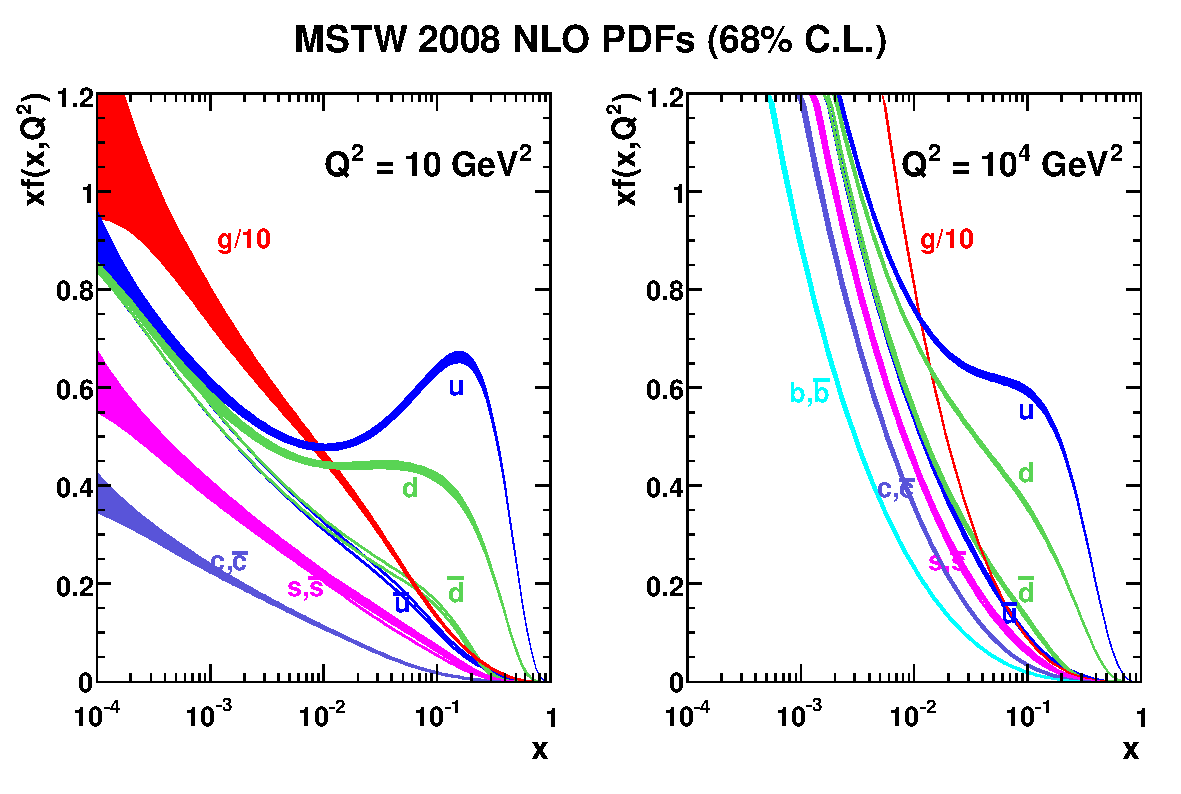
\includegraphics[width=0.9\textwidth]{images/pdfs.pdf}
  \caption{Typical momentum fraction distributions of partons inside the proton at a factorisation scale of \(Q^2 = 10\,\text{GeV}^2\). The plot shows the gluon and the first two generations of quarks, including valence components \(u_V\) and \(d_V\)~\cite{Martin_2009}.}
  \label{fig:pdfs}
\end{figure}

\subsubsection*{Parton-parton scattering}
\label{subsubsec:proton}
From these principles, the cross-sections for the processes that unfold at hadron colliders can be factorized into two contributions. The \acrshort{pdf}s describe the colliding partons $i$, $j$, within the colliding hadrons $H_{1}$, $H_{2}$. In the collision, the hard scattering process of interest corresponds to the short-distance interaction between both partons, each carrying a fraction of the parent hadrons's momentum. These interactions are characterised by a large momentum transfer and are described within the framework of perturbative \acrshort{qcd}. However, the collision environment also includes soft interactions with low momentum transfer, collectively referred to as the underlying event (UE), which encompasses remnants of the hadron-hadron system as well as potential multi-parton interactions (MPI), which are cases where more than one partonic interaction occurs within a single event.

Radiative processes such as Bremsstrahlung are inherent to high-energy collisions due to the acceleration of colour and electric charges. Initial State Radiation (ISR) arises from the incoming partons before the hard interaction, while Final State Radiation (FSR) originates from the outgoing partons. Following the hard interaction, partons undergo hadronisation, a non-perturbative \acrshort{qcd} process in which coloured partons are confined into colour-singlet hadrons. These hadrons are typically collimated into jets, observable in the detector.

Hence, the total cross-section for a given final state $X$ in a $pp$ collision is obtained via the factorisation theorem~\cite{fact_them,collins2004factorizationhardprocessesqcd}:
\begin{equation}
\sigma_{AB \to X} = \sum_{a,b} \int \mathrm{d}x_a \, \mathrm{d}x_b \, f_{a/A}(x_a, \mu_F^2) \, f_{b/B}(x_b, \mu_F^2) \, \hat{\sigma}_{ab \to X}(\hat{s}, \mu_R^2),
\end{equation}
where $f_{a/A}$ and $f_{b/B}$ are the \acrshort{pdf}s containing the non-perturbative component of the soft interaction, $\mu_F$ is the factorisation scale, and $\mu_R$ the renormalisation scale associated with the running of $\alpha_s$. The partonic cross-section $\hat{\sigma}$ is computed as a perturbative expansion in $\alpha_s(\mu_R)$:
\begin{equation}
\hat{\sigma}_{ab \to X} = \hat{\sigma}_0 + \alpha_s(\mu_R^2)\, \hat{\sigma}_1 + \alpha_s^2(\mu_R^2)\, \hat{\sigma}_2 + \cdots.
\end{equation}

While leading order (LO) calculations offer basic estimates, they suffer from large theoretical uncertainties due to strong dependence on $\mu_F$ and $\mu_R$. Higher-order corrections at next-to leading order (NLO) or next-to-next-to leading order (NNLO) reduce this dependence and yield more accurate predictions. The impact of these corrections is often quantified via the $K$-factor, defined as the ratio of the NLO to LO cross-sections.

%----------------------------------------------
\subsection{Electroweak Theory and Gauge Unification}
\label{subsec:ew_theory}
%----------------------------------------------

The electroweak (\acrshort{ew}) theory unifies the weak and electromagnetic interactions within a single gauge framework. It is formulated as a non-Abelian gauge theory based on the symmetry group $SU(2)_L \times U(1)_Y$, where $SU(2)_L$ accounts for weak isospin and $U(1)_Y$ for weak hypercharge. The theory was developed independently by Glashow, Weinberg, and Salam~\cite{Glashow,Weinberg,Salam}, and constitutes a central component of the Standard Model. The electroweak Lagrangian can be written as:

\begin{equation}
\begin{split}
\mathcal{L}_{\text{EW}} = 
&\sum_{flavours} i(\bar{L}\gamma^\mu D_\mu L +\bar{Q}\gamma^\mu D_\mu Q + \bar{l}_{R}\gamma^\mu D_\mu l_{R} + \bar{u}_{R}\gamma^\mu D_\mu u_{R} + \bar{d}_{R}\gamma^\mu D_\mu d_{R}) \\
&- \frac{1}{4} W_{\mu\nu}^a W^{a\,\mu\nu} - \frac{1}{4} B_{\mu\nu} B^{\mu\nu}
\end{split}
\label{eq:ew_lagrangian}
\end{equation}

The gauge fields associated with $SU(2)_L$ are denoted by $\vec{W}_\mu = (W_\mu^1, W_\mu^2, W_\mu^3)$, while the gauge field corresponding to $U(1)_Y$ is $B_\mu$. The corresponding gauge couplings are $g$ and $g'$, respectively. The covariant derivative acting on fermion fields is given by:
\begin{equation}
D_\mu = \partial_\mu - i \, g \, \frac{\vec{\tau}}{2} \cdot \vec{W}_\mu - i \, g' \, \frac{Y}{2} B_\mu,
\end{equation}
where $\vec{\tau}$ are the Pauli matrices and $Y$ is the weak hypercharge of the field.

Left-handed fermions are arranged in $SU(2)_L$ doublets, while right-handed fermions transform as singlets. For instance, the first-generation leptons are written as:
\begin{equation}
L_e =
\begin{pmatrix}
\nu_e \\
e
\end{pmatrix}_L, \qquad e_R,
\end{equation}
with $L_e$ transforming as a doublet under $SU(2)_L$ and $e_R$ as a singlet. It similarly applies to left-handed quark doublets, $Q$, and singlets, $u$ and $d$. The weak hypercharges are assigned such that the electric charge $Q$ of each field is given by the Gell-Mann–Nishijima relation:
\begin{equation}
Q = T_3 + \frac{Y}{2},
\end{equation}
where $T_3$ is the third component of weak isospin.

The kinetic term of the gauge fields is given by:
\begin{equation}
\mathcal{L}_{\text{gauge}} = -\frac{1}{4} \, \vec{W}_{\mu\nu} \cdot \vec{W}^{\mu\nu} - \frac{1}{4} \, B_{\mu\nu} B^{\mu\nu},
\end{equation}
where the field strength tensors are defined as:
\begin{align}
W_{\mu\nu}^i &= \partial_\mu W_\nu^i - \partial_\nu W_\mu^i + g \, \epsilon^{ijk} W_\mu^j W_\nu^k, \\
B_{\mu\nu} &= \partial_\mu B_\nu - \partial_\nu B_\mu.
\end{align}

Fermion interactions with the gauge bosons arise from the kinetic term of the fermion fields:
\begin{equation}
\mathcal{L}_{\text{fermion}} = \sum_{\psi} \bar{\psi} \, i \slashed{D} \, \psi,
\end{equation}
leading to charged and neutral current interactions. The charged currents couple only to left-handed fermions via $W^\pm$ bosons (linear combinations of $W^1$ and $W^2$), while neutral currents arise from couplings to $W^3$ and $B$.

At this stage, all gauge bosons and fermions are massless. Mass terms are forbidden by gauge invariance, and it is only through spontaneous symmetry breaking that physical masses are generated, as discussed in the next section. Additionally, the structure of the theory prior to breaking ensures parity violation in weak interactions due to the chiral nature of the $SU(2)_L$ coupling.

This unbroken \acrshort{ew} theory thus describes the fundamental structure of weak and electromagnetic interactions prior to the introduction of the Higgs field, which provides masses to the gauge bosons and fermions while preserving gauge invariance through the Higgs mechanism.

%----------------------------------------------
\subsection{Spontaneous Symmetry Breaking and the Higgs Mechanism}
\label{subsec:higgs_mech}
%----------------------------------------------

In order to generate the mass of weak vector bosons and fermions while preserving renormalizability and unitarity, the Standard Model introduces a Spontaneous Symmetry Breaking mechanism in the electroweak theory. 
This mechanism is referred to as the Brout–Englert–Higgs (\acrshort{beh}) mechanism~\cite{Brout,HiggsSpontan}, and it introduces a complex scalar field doublet $\phi$ with hypercharge $Y=+1$, whose dynamics are governed by the gauge-invariant Lagrangian:
\begin{equation}
\mathcal{L}_\phi = (D_\mu \phi)^\dagger(D^\mu \phi) - V(\phi),
\end{equation}
where $V(\phi)$ is the scalar potential:
\begin{equation}
V(\phi) = \mu^2 \phi^\dagger \phi + \lambda(\phi^\dagger \phi)^2,
\label{eq:higgs_potential}
\end{equation}
with $\lambda > 0$ ensuring the potential is bounded from below. The sign of $\mu^2$ determines the nature of the vacuum: for $\mu^2 > 0$, the potential has a single minimum at $\phi = 0$, preserving the gauge symmetry. However, for $\mu^2 < 0$, the potential takes the shape of a “Mexican hat”, as illustrated in Figure~\ref{fig:mexican_hat}, with a continuous set of degenerate minima.

Since the Lagrangian is gauge invariant, the Higgs field can be described using an exponential decomposition:
\begin{equation}
\phi(x) = \frac{1}{\sqrt{2}} \, e^{i \tau_{a} \theta^a(x)/f} \begin{pmatrix}
0 \\
\rho(x)
\end{pmatrix},
\label{eq:higgs_param}
\end{equation}
where $\theta^a(x)$ and $\rho(x)$ are real fields, $\tau_{a}$ are the SU(2) generators\footnote{Elements of the group that generate the group when combined with themselves using the group's operations}, and $f$ is a normalisation constant.

One of the degenerate minima can be chosen without loss of generality as:
\begin{equation}
\langle \phi \rangle = \frac{1}{\sqrt{2}} \begin{pmatrix}
0 \\
v
\end{pmatrix},
\end{equation}
which spontaneously breaks the $SU(2)_L \times U(1)_Y$ gauge symmetry down to the electromagnetic subgroup $U(1)_{\text{EM}}$.

\begin{figure}[htbp]
  \centering
  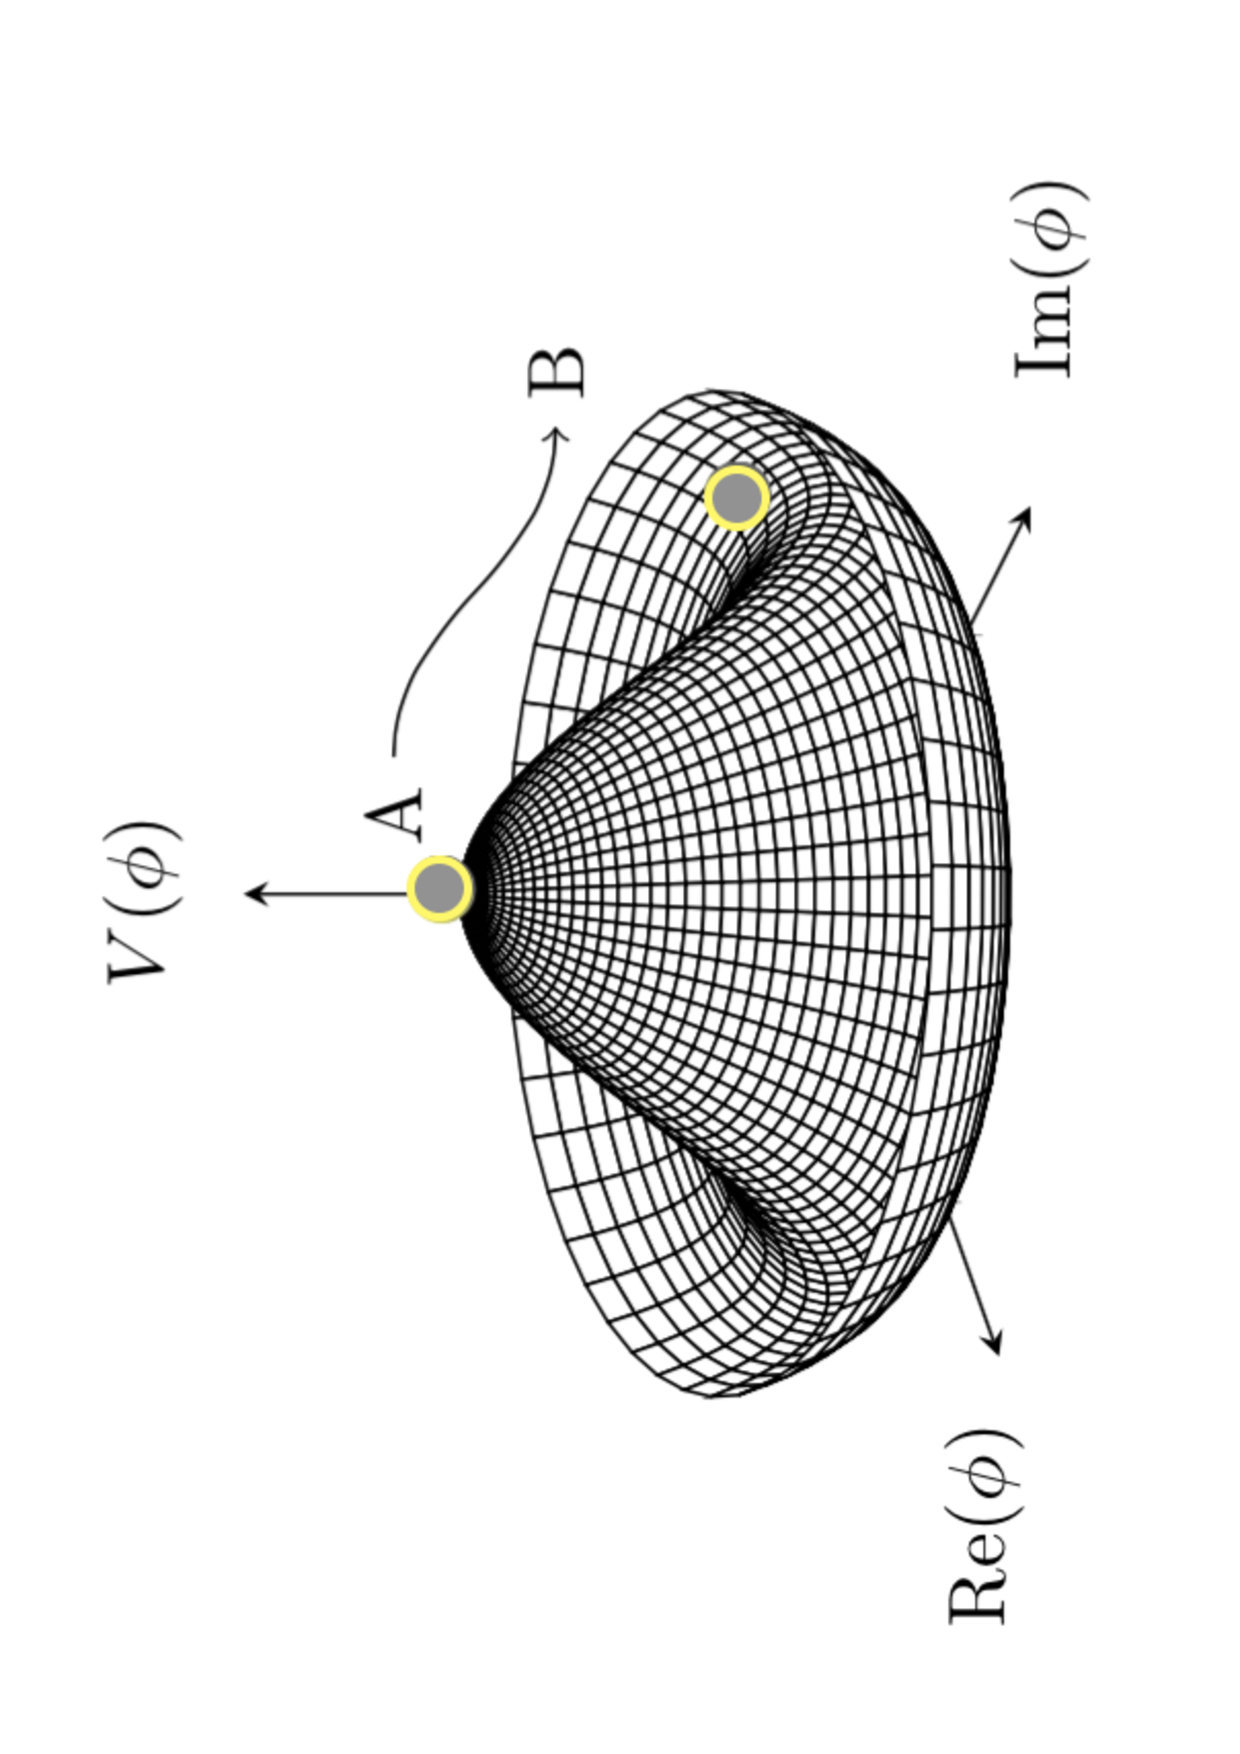
\includegraphics[angle=-90,width=0.7\textwidth]{images/mexican_hat.pdf}
  \caption{Illustration of the shape of the Higgs complex scalar potential with vacuum expectation value $v$. The symmetry is spontaneously broken when a singular ground state is chosen (A $\rightarrow$ B).}
  \label{fig:mexican_hat}
\end{figure}

The simplest way to expand the Higgs field is to keep the minimum number of degrees of freedom, so replacing $v\rightarrow v+h(x)$ in the previous equation and substituing in the potential Lagrangian (Eq.~\ref{eq:higgs_potential}): 

\begin{equation}
\begin{split}
\mathcal{L}_{H} = 
&\frac{1}{2}(\partial_{\mu}h)(\partial^{\mu}h) + \frac{1}{2}(2\mu^2)h^2\\  
& + \frac{1}{2}\frac{g^2_{W}v^2}{4}(W_{\mu}^1W^{1\mu}+W_{\mu}^2W^{2\mu})\\
& +\frac{1}{8}v^2(g_{W}W^{3\mu}-g_{B}B^{\mu})\\ 
& + \mathcal{O}(h^2)
\end{split} 
\label{eq:ew_broken}
\end{equation}

This expression contains quadratic terms interpreted as the mass terms of the particles associated to the fields. Since gauge boson terms here are not linearly independent, they cannot be interpreted as observables. Physical bosons can be obtained diagonalizing this sector, resulting in:
\begin{align}
W^\pm_\mu &= \frac{1}{\sqrt{2}} \left( W^1_\mu \mp i W^2_\mu \right), \\
Z_\mu &= \cos\theta_W W^3_\mu - \sin\theta_W B_\mu, \\
A_\mu &= \sin\theta_W W^3_\mu + \cos\theta_W B_\mu,
\end{align}
where $\theta_W$ is the weak mixing angle defined by $\tan \theta_W = g_B /g_W$.
Using these definitions, the corresponding masses of the gauge bosons can be obtained from the Lagrangian as follows:
\begin{align}
m^{\pm}_W &= \frac{1}{2} g v, \\
m_Z &= \frac{1}{2} \sqrt{g^2 + g'^2} \, v, \\
m_\gamma &= 0,
\end{align}
where $v = 246 \text{  GeV}$ is the Higgs field vacuum expectation value and g is the weak isospin coupling constant. 
This mechanism results in two massive vector bosons $W^{\pm}$ which corresponds to the weak charged current, and other massive boson Z, carrier of the neutral weak current. It also remains a massless gauge boson, $A_{\mu}$, which corresponds to the photon and is consistent with the unbroken \acrshort{qed} symmetry $U(1)$.

From eq.~\ref{eq:ew_broken}, the mass term for the scalar field $H$ turns to be:
\begin{equation}
m_H^2 = 2 \mu^2,
\end{equation}
where it depends on the free parameter $\mu^2$ that can be experimentally measured and it has been done with \acrshort{lhc} Run 1 and Run 2 data by ATLAS and CMS~\cite{ATLASCMS}:
\begin{equation}
m_H = 125.09 \pm 0.24 \text{ GeV}
\end{equation}

Moreover, the \acrshort{beh} mechanism can also be used to provide mass terms for the fermions preserving the gauge invariance of the theory.
Adding the Yukawa terms~\cite{Peskin} describing fermion couplings to the Higgs field into the \acrshort{ew} Lagrangian, one gets:
\begin{equation}
\mathcal{L}_{\text{Yukawa}} = 
\sum_{\text{flavours}} \left( 
- \lambda_\ell \, \bar{L} \phi \ell_R 
- \lambda_d \, \bar{Q} \phi d_R 
- \lambda_u \, \epsilon^{ab} \, \bar{Q}_a \phi_b^{\dagger} u_R 
+ \text{h.c.} 
\right)
\end{equation}
where $\lambda_{e}$, $\lambda_{d}$ and $\lambda_{u}$ are arbitrary parameters and $\epsilon^{ab}$ is the two dimensional total anti-symmetric tensor with $\epsilon^{12}=1$. After symmetry breaking we get the following mass terms for the fermion fields after proper diagonialization: 
\begin{equation}
m_{l}=\lambda_{l}\frac{v}{\sqrt{2}}, \ m_{d}=\lambda_{d}\frac{v}{\sqrt{2}}, \ m_{u}=\lambda_{u}\frac{v}{\sqrt{2}},
\end{equation}
from where the Yukawa coupling strength of fermions to the Higgs field can be defined as
\begin{equation}
\label{yukawa}
y_{f}=\sqrt{2}\frac{m_{f}}{v}
\end{equation}
Moreover, these fermion mass eigenstates and the weak eigenstates are related via the $3x3$ unitary Cabibbo-Kobayashi-Maskawa (\acrshort{ckm}) matrix, $V_{CKM}$,
\begin{equation}
\begin{pmatrix}
d^0 \\
s^0 \\
b^0
\end{pmatrix}
= V_{\text{CKM}}
\begin{pmatrix}
d \\
s \\
b
\end{pmatrix}
=\begin{pmatrix}
V_{ud} & V_{us} & V_{ub} \\
V_{cd} & V_{cs} & V_{cb} \\
V_{td} & V_{ts} & V_{tb}
\end{pmatrix}
\begin{pmatrix}
d \\
s \\
b
\end{pmatrix},
\end{equation}
where the off-diagonal elements cause flavour changing weak charged current interactions of quarks with their transition probabilities being proportional to $|V_{nm}|^2$.

%++++++++++++++++++++++++++++++++++++++++++++++
\section{Success and fundamental limitations of the SM}
\label{sec:BSM}
%++++++++++++++++++++++++++++++++++++++++++++++
After integrating all the essential elements forming the Standard Model, the theory is characterized by nineteen undetermined parameters:
\begin{itemize}
  \item a total of nine Yukawa couplings corresponding to the three charged leptons and six quarks,
  \item three gauge coupling constants governing the strengths of the interactions: \( g_s \), \( g \), and \( g' \),
  \item two parameters characterizing the Higgs potential: the vacuum expectation value \(\nu\) and the Higgs boson mass \(m_H\),
  \item four resulting mixing angles defining the structure of the \acrshort{ckm} matrix,
  \item a single strong CP-violating phase \(\theta_{CP}\), which is conventionally assumed to be zero, implying the absence of CP violation in strong interactions.
\end{itemize}
Despite being defined by only 19 free parameters, the Standard Model has demonstrated extraordinary predictive power, with theoretical predictions consistently matching experimental results over several decades. This success is exemplified in Figure~\ref{fig:totalxsect}, which presents the cross-sections measured by the ATLAS experiment for a variety of processes occurring across multiple orders of magnitude.
\begin{figure}[htbp]
  \centering
  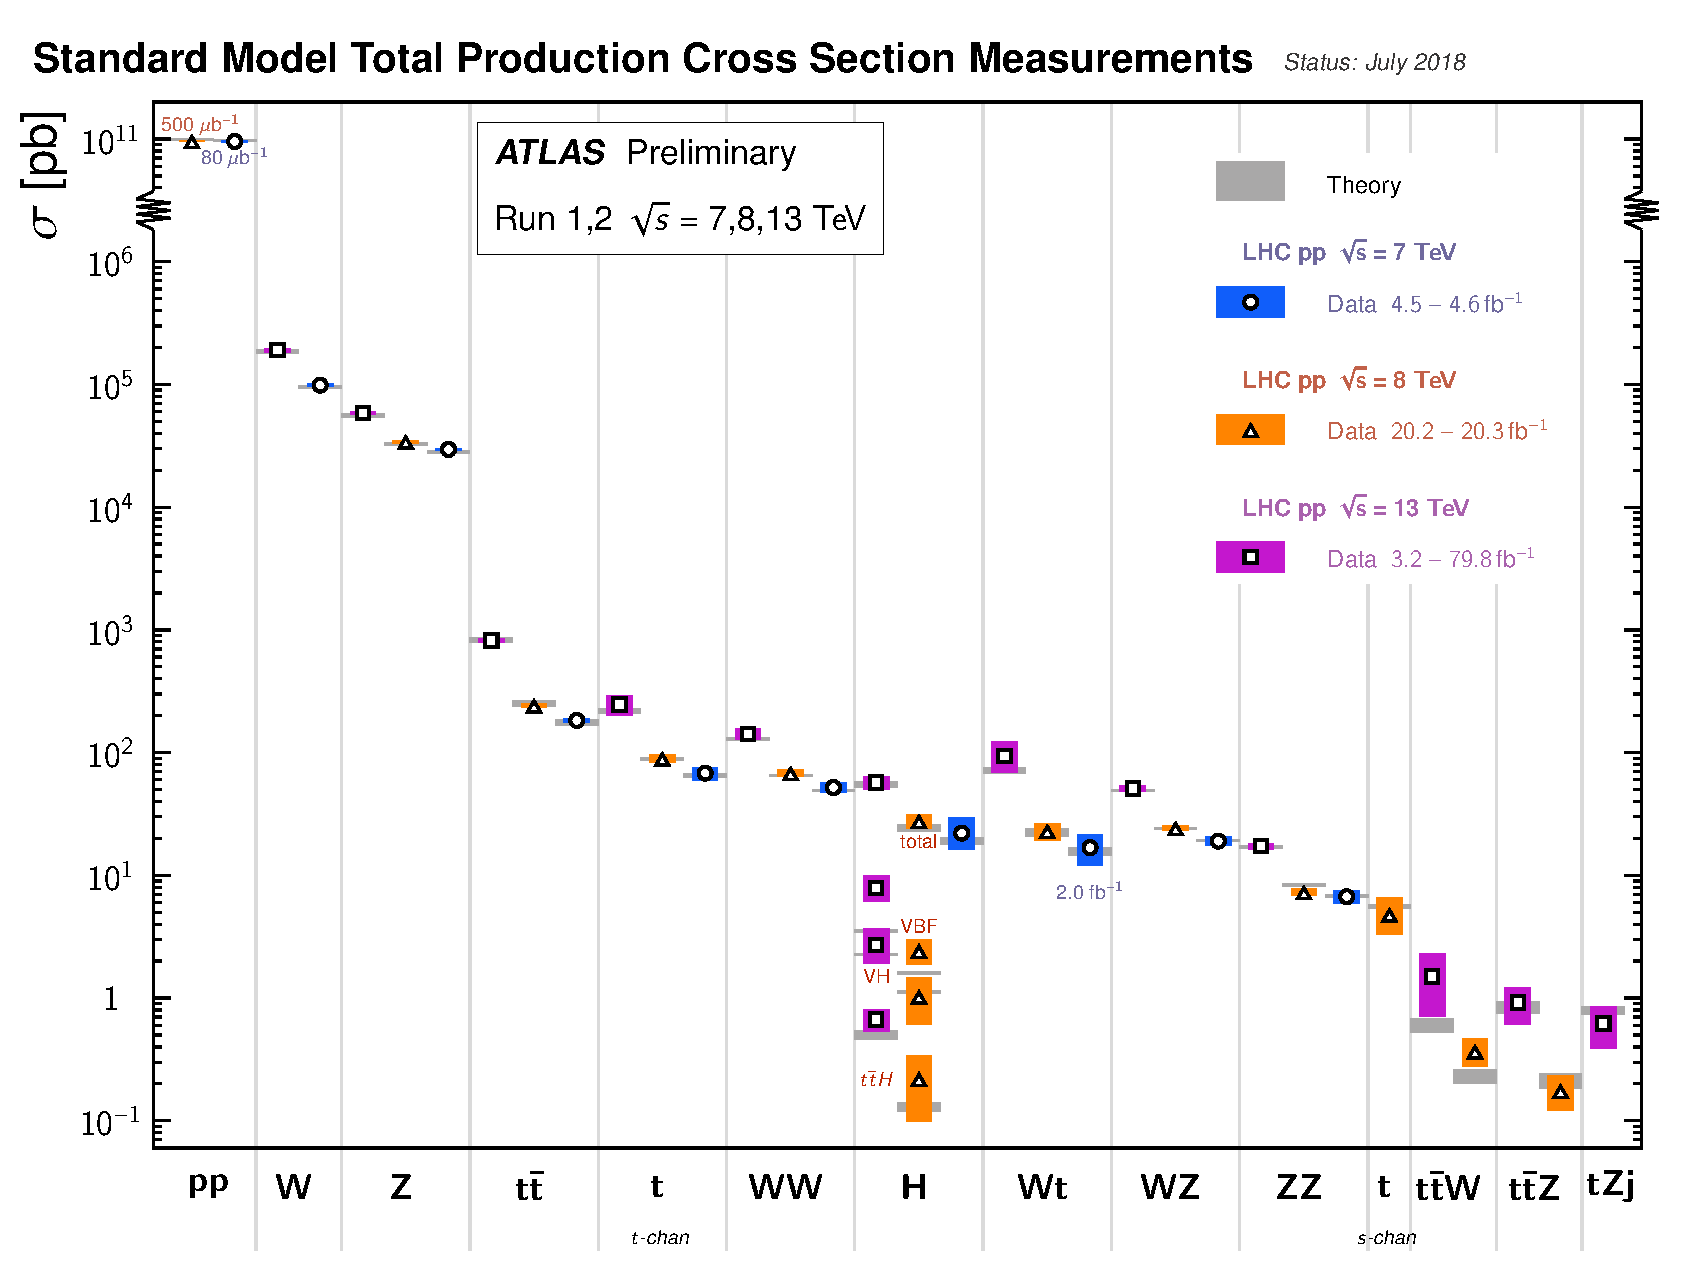
\includegraphics[width=0.8\textwidth]{images/totalxsect.pdf}
  \caption{Summary of several Standard Model total production cross-section measurements, compared to the corresponding theoretical expectations. All theoretical expectations were calculated at NLO or higher~\cite{PlotsXsect}.}
  \label{fig:totalxsect}
\end{figure}

\subsection*{Open questions}

Despite its remarkable success, the \acrshort{sm} is not considered a complete theory of fundamental interactions. Some of the most relevant issues that this theory does not address are listed here:
\subsubsection*{Dark Matter}

Astrophysical and cosmological observations provide compelling evidence for the existence of dark matter (\acrshort{dm}), a form of non-luminous matter not accounted for in the Standard Model. Measurements of galactic rotation curves, gravitational lensing in galaxy clusters (e.g., the Bullet Cluster~\cite{Clowe_2006}), and the cosmic microwave background anisotropies consistently indicate that approximately 85\% of the matter content of the universe is non-baryonic~\cite{Planck}. While several extensions of the Standard Model propose viable \acrshort{dm} candidates, such as weakly interacting massive particles (\acrshort{wimp}) or axions, the \acrshort{sm} itself does not provide a suitable particle to explain these phenomena.

\subsubsection*{Neutrino Masses and Oscillations}

Experimental evidence from solar, atmospheric, reactor, and accelerator neutrino experiments has firmly established that neutrinos undergo flavor oscillations, implying they have non-zero masses and mixings~\cite{PhysRevD.98.030001}. This observation requires the existence of mass terms beyond the Standard Model's original framework, which assumes massless neutrinos. Mechanisms such as the seesaw model, introducing right-handed neutrinos or Majorana mass terms, are common in theories beyond the \acrshort{sm}, but are not present in its minimal formulation.

\subsubsection*{Matter-Antimatter Asymmetry}

The observed universe is dominated by matter over antimatter, a phenomenon known as baryon asymmetry. While the Standard Model includes a source of CP violation through the complex phase in the \acrshort{ckm} matrix, it is insufficient to account for the observed phenomena. Additional sources of CP violation and new physics at high energy scales are required to explain this asymmetry.

\subsubsection*{Hierarchy Problem}

The mass of the Higgs boson receives large quantum corrections proportional to the square of the energy cutoff scale of the theory. Stabilizing the Higgs mass at the electroweak scale without unnatural fine-tuning requires a mechanism to cancel these divergences. Supersymmetry, composite Higgs models, and extra-dimensional theories have been proposed as potential solutions, but no evidence of such physics has yet been observed.

\subsubsection*{Gravity and the Lack of Unification}

The Standard Model does not incorporate gravity, which is described by General Relativity. Moreover, the gauge couplings of the \acrshort{sm} do not unify at a single energy scale, unless new physics (e.g., supersymmetry) is introduced. A complete theory of fundamental interactions would require a quantum theory of gravity and a framework capable of unifying all known forces, such as string theory or grand unified theories (GUTs).

\subsubsection*{Vacuum Stability and the Top Quark Yukawa Coupling}
The stability of the (\acrshort{ew}) vacuum depends critically on the running of the Higgs self-coupling $\lambda$, governed by the renormalization group equations. Among all parameters, the top quark Yukawa coupling $y_t$ has the largest impact due to its sizeable contribution to the $\beta$-function of $\lambda$.

A large value of $y_t$ tends to drive $\lambda$ to negative values at high energy scales, which would imply that the \acrshort{ew} vacuum is only metastable, with a deeper minimum appearing at large field values. In this case, our universe resides in a long-lived but not absolutely stable vacuum. Current measurements of $m_H$, $\alpha_s$, and especially $m_t$ suggest that this is indeed the case.

The precise value of $y_t$, and thus the top quark mass, is crucial: small shifts can determine whether the vacuum is stable, metastable, or unstable. Accurate measurements of processes such as $t\bar{t}H$ production are therefore essential not only for testing the Standard Model but also for probing its validity up to the Planck scale.


%++++++++++++++++++++++++++++++++++++++++++++++
\section{Phenomenology of the Top Quark and the Higgs Boson at the LHC}
\label{sec:top_higgs_lhc}
%++++++++++++++++++++++++++++++++++++++++++++++
The top quark and the Higgs boson play a central role in the (\acrshort{sm}) and in the exploration of physics beyond it. Their large masses, unique interactions, and profound implications for electroweak symmetry breaking and vacuum stability make them particularly interesting from both theoretical and experimental perspectives. 

%xxxxxxxxxxxxxxxxxxxxxxxxxxxxxxxxxxxxxxxxxxxxxxxxxxxxxx
\subsection{The Top quark}
\label{sec:top_quark}
%xxxxxxxxxxxxxxxxxxxxxxxxxxxxxxxxxxxxxxxxxxxxxxxxxxxxxx

The top quark, proposed by Kobayashi and Maskawa in 1973~\cite{10.1143/PTP.49.652} and discovered at the Tevatron in 1995~\cite{PhysRevLett.74.2626,PhysRevLett.74.2632} is the heaviest known elementary particle, with a mass around $173$ GeV. This them to decay into $W$ bosons and $b$ quarks, which always happens before they can form hadrons. They can also decay into other down-type quarks, but due to the \acrshort{ckm} matrix, this is practically negligible in practice. Due to its large mass, the top quark has a Yukawa coupling almost equal to unity.

\subsubsection*{Top quark production}
\label{subsec:top_quark_prod}
At hadron colliders such as the \acrshort{lhc}, the top quark production mostly ocurrs in pairs ($t\bar{t}$) through the strong interaction. At \acrshort{lo}, the two leading subprocesses are gluon-gluon fusion (\acrshort{ggf}) and $q\bar{q}$ annihilation, as represented in Figure~\ref{fig:tt-production}. Gluon fusion accounts for roughly $90\%$ of the total $t\bar{t}$ cross-section at a centre-of-mass energy of 13 TeV, which is the practical scenario when protons collide at \acrshort{lhc} where gluon parton densities are dominant. 
\begin{figure}[htbp]
    \centering


        \centering
        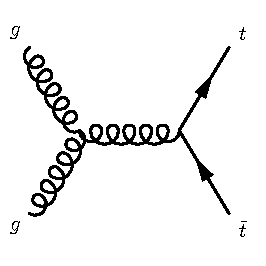
\includegraphics[width=0.3\textwidth]{feyn_gg_ttbar_1.pdf}
        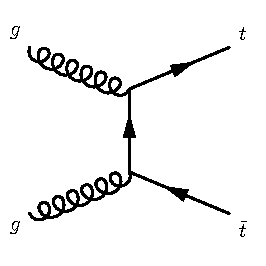
\includegraphics[width=0.3\textwidth]{feyn_gg_ttbar_2.pdf}
        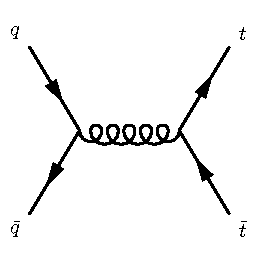
\includegraphics[width=0.3\textwidth]{feyn_qq_ttbar.pdf}
    

    \caption{Leading-order Feynman diagrams contributing to top quark pair production in hadron colliders. The dominant process at the \acrshort{lhc} is gluon-gluon fusion, first and second from the left, while quark-antiquark annihilation (third) dominates at lower center-of-mass energies (Tevatron).}
    \label{fig:tt-production}
\end{figure}

Nevertheless, top quarks can also be produced singly via the electroweak interaction, either alone or in association with other particles. Single-top has a much smaller cross-section, but processes like t$W$ or \tH also encapsulate important complementary information.
Among all of them, \tH and \ttH play a central role in this thesis by forming the signal processes that are discussed in the last chapters of the thesis. They will be futher covered in more detail at the end of this chapter.

\subsubsection*{Top-antitop system decay}
\label{subsec:top_quark_decay}

As mentioned, top quarks are mainly produced at hadron colliders in $t\bar{t}$ pairs. Given that the top quark decays nearly the $100\%$ of cases as $t\rightarrow Wb$, the properties of $t\bar{t}$ final states mainly depend on how the $W$ boson decays, as it is shown in Figure~\ref{fig:diagram-and-table-top}.
\begin{figure}[htbp]
    \centering
    % Imagen a la izquierda (como subfigure)
    \begin{minipage}[c]{0.48\textwidth}
        \centering
        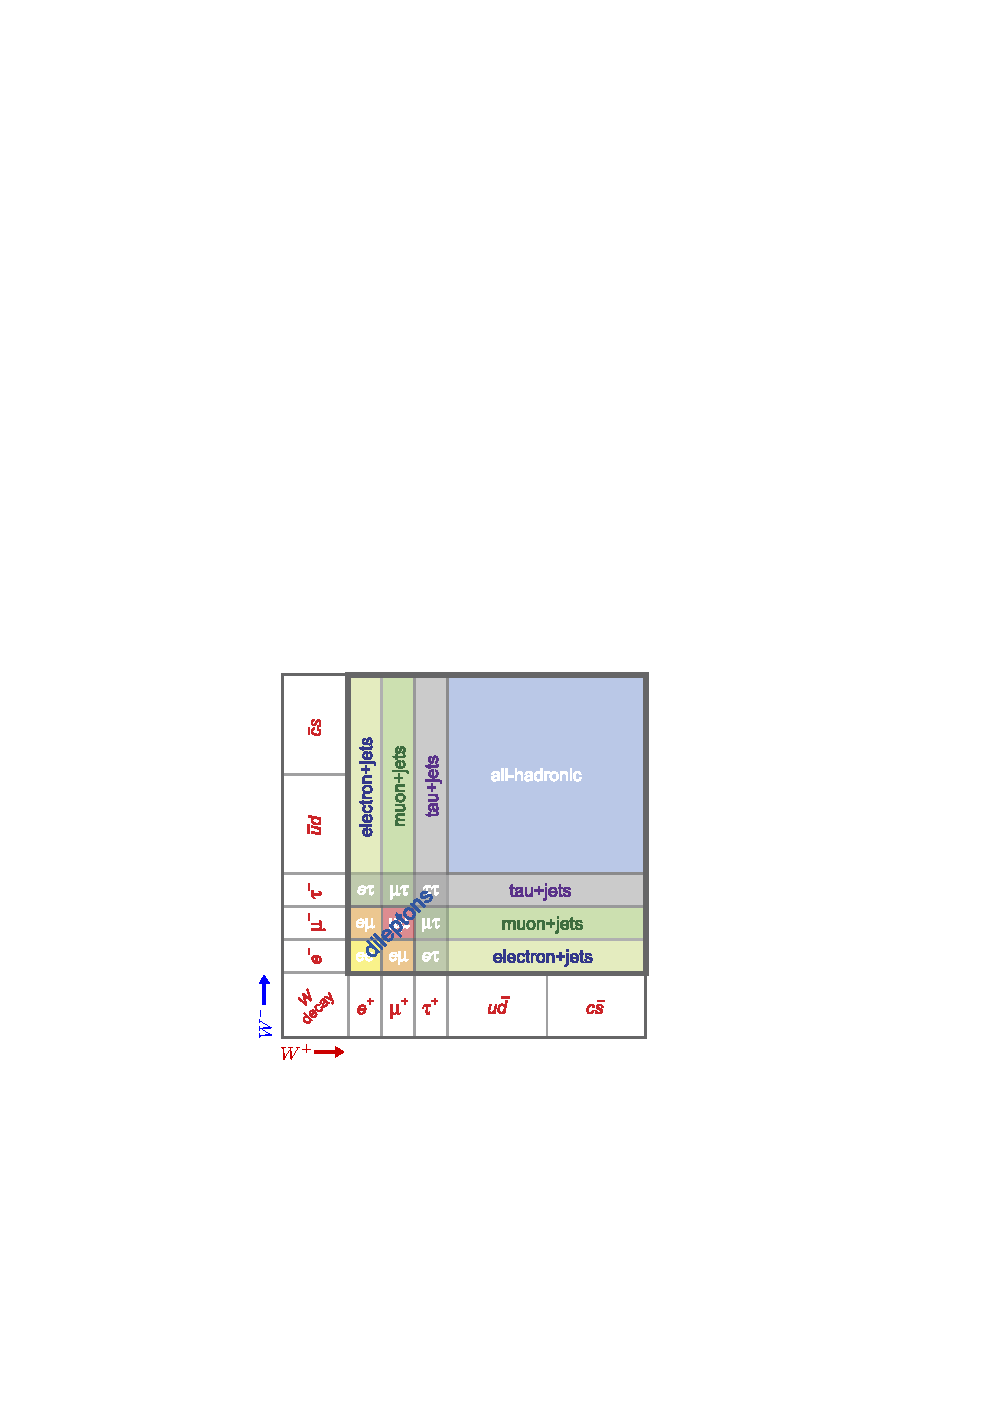
\includegraphics[width=\textwidth]{tt_decay_channels.pdf}
    \end{minipage}
    \hfill
    % Tabla a la derecha
    \begin{minipage}[c]{0.48\textwidth}
        \centering
        \footnotesize
        \begin{tabular}{ll}
            \hline
            \textbf{Final state} & \textbf{Branching fraction} \\ \hline
            all-hadronic         & 45.7\%                     \\
            semi-leptonic        & 43.8\%                     \\
            dileptonic           & 10.5\%                     \\\hline
        \end{tabular}
    \end{minipage}
    \caption{Left: classification of $t\bar{t}$ decay channels based on the $W$ decay modes~\cite{Lannon_2012}. Right: inclusive branching ratios for the $t\bar{t}$ system decay~\cite{ParticleDataGroup}.}
    \label{fig:diagram-and-table-top}
\end{figure}

The fully hadronic final state corresponds to the case where both $W$ bosons decay into quark-antiquark pairs. This is the most frequent decay mode. An smaller fraction of events corresponds to the semileptonic final state, in which one of the bosons decays hadronically, while the other decays leptonically producing a charged lepton and a neutrino. In the case of the dileptonic final state, both $W$ bosons decay into leptons.

The table in Figure~\ref{fig:diagram-and-table-top} considers $\tau$-leptons within the general category of leptons. However, in the context of physics analysis, it is common for the term "leptonic decay" to be used only to refer to decays into light charged leptons, i.e. electrons and muons, including those from the decay of $\tau$ leptons. For experimental reasons, hadronic decays of $\tau$-leptons are treated differently, as discussed in Section~\ref{sec:ttH}.

%xxxxxxxxxxxxxxxxxxxxxxxxxxxxxxxxxxxxxxxxxxxxxxxxxxxxxx
\subsection{The Higgs Boson in the LHC Physics Program}
\label{sec:higgs_program}
%xxxxxxxxxxxxxxxxxxxxxxxxxxxxxxxxxxxxxxxxxxxxxxxxxxxxxx

Since its discovery in 2012 by ATLAS and CMS~\cite{ATLAS:2012yve,CMS:2012qbp}, the Higgs boson has become a central component of the \acrshort{lhc} physics program. Its role in providing masses to the $W$ and $Z$ bosons through the Brout–Englert–Higgs mechanism, and subsequently to all fermions in nature, is a cornerstone of the \acrshort{sm}. Studying its properties in detail allows stringent tests of the \acrshort{sm} and provides sensitivity to B\acrshort{sm} scenarios.

The ATLAS and CMS experiments have undertaken a comprehensive program of Higgs boson measurements. These include the determination of its mass, spin and CP properties, as well as its couplings to fermions and bosons. The precision of these measurements continues to improve with each \acrshort{lhc} run, and new production and decay channels are explored regularly.

%xxxxxxxxxxxxxxxxxxxxxxxxxxxxxxxxxxxxxxxxxxxxxxxxxxxxxx
\subsubsection*{Higgs boson production mechanisms}
\label{sec:higgs_production}
%xxxxxxxxxxxxxxxxxxxxxxxxxxxxxxxxxxxxxxxxxxxxxxxxxxxxxx
The main production modes at tree level in which the Higgs boson can be produced at proton-proton collisions are presented in Figure~\ref{fig:higgs_production}. The right plot in Figure~\ref{fig:higgs_comb} shows the cross-section as a function of the centre-of-mass energy for a Higgs boson with mass $m_{H}=125$ GeV.

% Begin the figure
\begin{figure}[htbp]
    \centering
    % Primera fila: 3 imágenes centradas
    \begin{tabular}{ccc}
        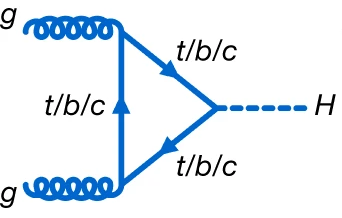
\includegraphics[width=0.3\linewidth]{images/ggF.png}  &
        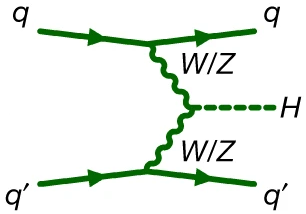
\includegraphics[width=0.3\linewidth]{images/VBF.png}  &
        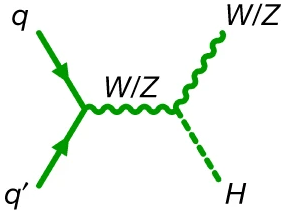
\includegraphics[width=0.3\linewidth]{images/VH.png}   \\
        (a) $ggF$ & (b) $VBF$ & (c) $VH$ \\
    \end{tabular}
    \vspace{0.5em} % Espacio entre filas
    % Segunda fila: 2 imágenes centradas bajo las 3 primeras
    \makebox[\textwidth][c]{%
        \begin{tabular}{cc}
            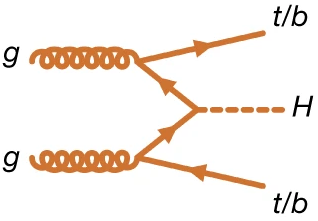
\includegraphics[width=0.3\linewidth]{images/ttH.png} &
            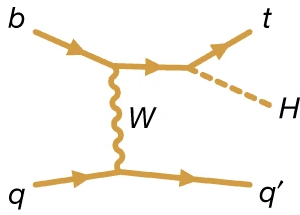
\includegraphics[width=0.3\linewidth]{images/tH.png} \\
            (d) $t\bar{t}(b\bar{b})H$ & (e) $tH$ \\
        \end{tabular}%
    }
    \caption{
    Examples of leading order Feynman diagrams for Higgs-boson production modes at the \acrshort{lhc}~\cite{Nature_ATLAS}.}
    \label{fig:higgs_production}
\end{figure}

\begin{figure}[htbp]
        \centering
        \begin{tabular}{cc}
        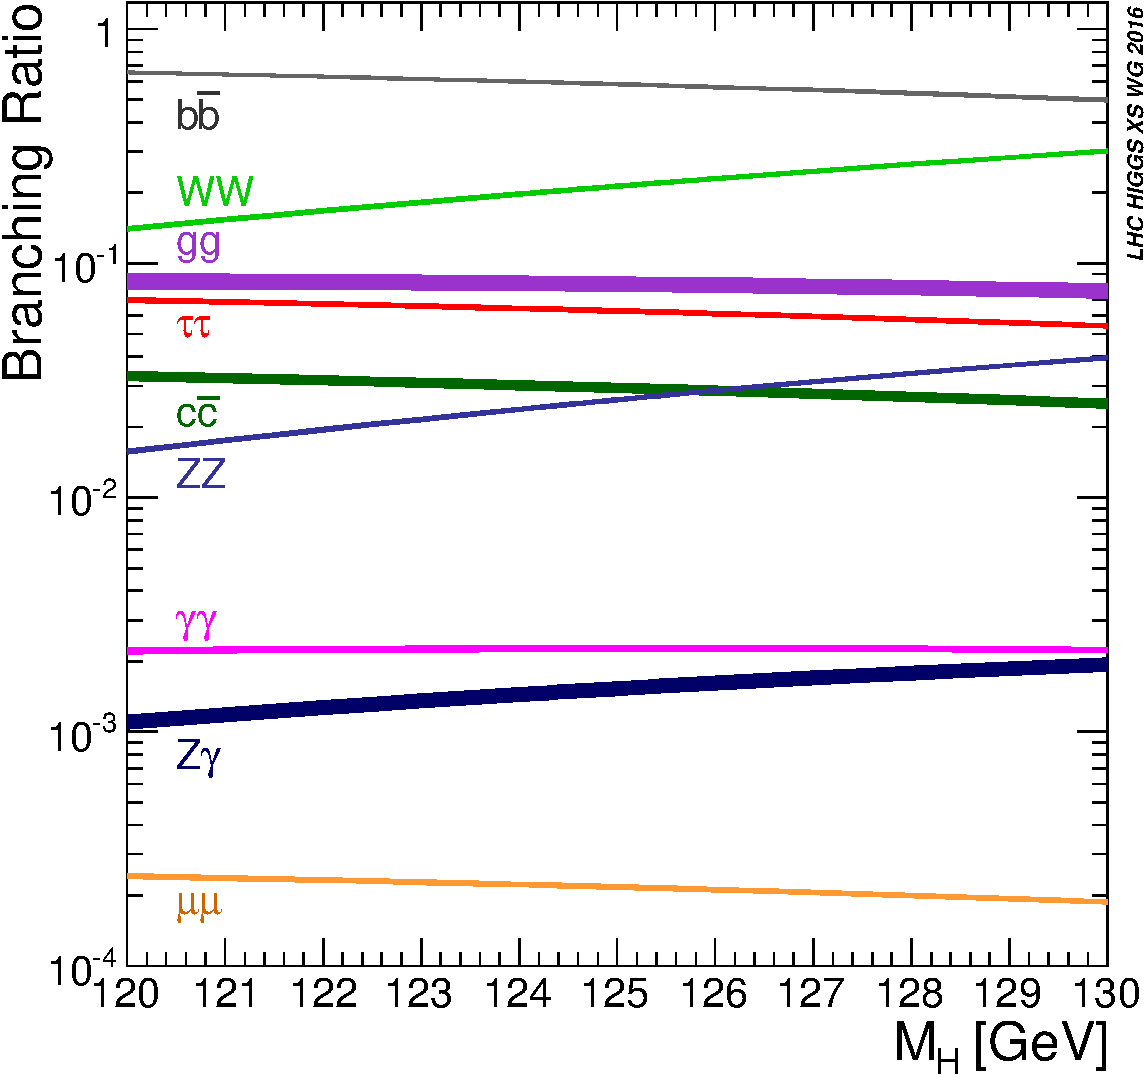
\includegraphics[width=0.46\textwidth]{images/higgs_dec.pdf} & 
        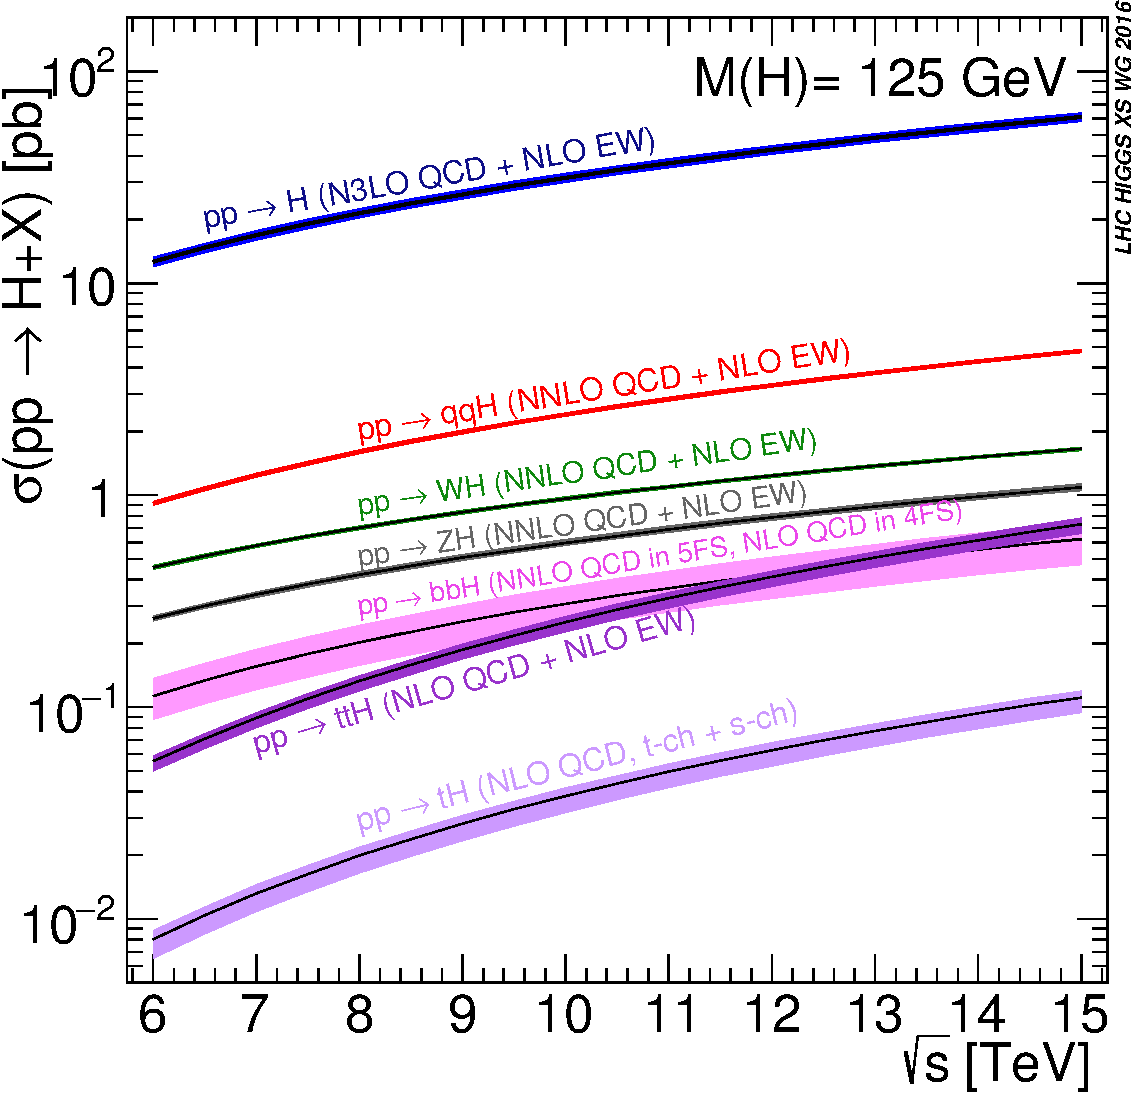
\includegraphics[width=0.46\textwidth]{images/higgs_prod.pdf}
        \end{tabular}
        \caption{ (a) Cross-sections measured for Higgs boson production at center of mass energy of 13 TeV as a function
        of the Higgs boson mass. (b) Branching ratios for the different Higgs boson decay modes as a function of the Higgs boson mass~\cite{Nature_ATLAS}}
        \label{fig:higgs_comb}
    \end{figure}

The dominant production mode is gluon-gluon fusion, where two gluons from the colliding protons interact via a heavy quark loop, primarily involving the top quark, to produce a Higgs boson. This process accounts for about 90\% of the total Higgs boson production cross-section at a centre-of-mass energy of 13 TeV, due to the high gluon density within the proton.

Another important channel is vector boson fusion (VBF), responsible of $6.8\%$ of the total cross-section. The Higgs boson is produced via a $t$-channel exchange of two weak bosons radiated from the incoming quarks, being this mechanism characterized by the presence of two high-momentum hard jets emitted at small angles from the colliding protons, while the Higgs is tipically produced between them in the central region, offering a clean and efficient experimental signature. 

Associated production with a vector boson (VH), also called "Higgs-strahlung", where the Higgs is produced alongside a $W$ or $Z$ boson, is particularly useful in final states with leptons, providing strong handles for background discrimination in a hadronic environment. It provides around the $4\%$ of the Higgs cross-section.

Finally, the associated production with a pair of top quarks ($t\bar{t}H$) provides a direct probe of the Yukawa coupling between the Higgs and the top quark, the strongest coupling in the \acrshort{sm}. Although its cross-section is significantly lower than other channels, around the $0.92\%$, it plays a strategic role in testing the interaction responsible for the top quark mass generation, which will be discussed in the following.
The rarest considered production mode is the associated production with a single top quark, accouting for a $0.16\%$. This process could also contribute to the determination of the direct top quark Yukawa coupling. However, its cross-section is significantly smaller than that of \( t\bar{t}H \) production. Furthermore, additional \acrshort{lo} diagrams for \( tH \) production involve the \( W \)-Higgs coupling, which already blurs the measurement. It is also worth noting that this process is sensitive to the sign of the top quark Yukawa coupling, which causes the interference between the dominant contributing channels to be destructive, hence its small cross-section.

Additionally, there are other production modes that remain experimentally challenging, such as Higgs boson production in association with bottom quark pairs, \( b\bar{b}H \). While this mode has a cross-section comparable to that of \( t\bar{t}H \), it suffers from a much less clean experimental signature due to the large background contribution from \acrshort{qcd} processes.

%xxxxxxxxxxxxxxxxxxxxxxxxxxxxxxxxxxxxxxxxxxxxxxxxxxxxxx
\subsubsection*{Higgs boson decay modes}
\label{sec:higgs_decay}
%xxxxxxxxxxxxxxxxxxxxxxxxxxxxxxxxxxxxxxxxxxxxxxxxxxxxxx

The \acrshort{sm} Higgs boson, with a lifetime of approximately \(10^{-22}\) seconds, decays into a wide range of experimentally accessible final states that enable its observation, as its extremely short existence precludes direct detection.

As mentioned in Section~\ref{subsec:higgs_mech}, the coupling of the Higgs boson to fermions is proportional to the fermion mass, while for gauge bosons the coupling is proportional to \(m_Z^2\) and \(m_W^2\) in the \(HZZ\) and \(HWW\) vertices, respectively. Consequently, the Higgs boson decays preferentially into the heaviest particles kinematically allowed.

Figure~\ref{fig:higgs_comb} shows the predicted branching ratios for the decay of the \acrshort{sm} Higgs boson as a function of its mass. In what follows, we focus on the branching ratios (\(\mathcal{B}\)) extracted from the ParticleDataGroup~\cite{ParticleDataGroup} for a Higgs boson with a mass of \(m_H = 125.09~\mathrm{GeV}\). Representative Feynman diagrams for the dominant decay modes are displayed in Figure~\ref{fig:h_decays}.

% Begin the figure
\begin{figure}[htbp]
    \centering
    % Primera fila: 3 imágenes centradas
    \begin{tabular}{ccc}
        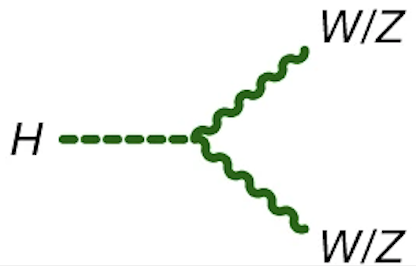
\includegraphics[width=0.3\linewidth]{images/HVV.png}  &
        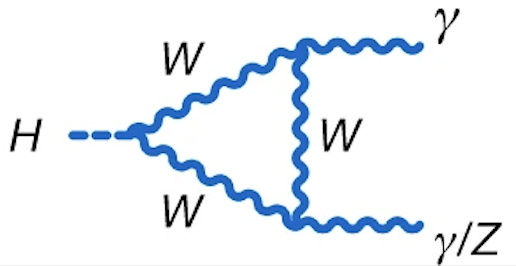
\includegraphics[width=0.3\linewidth]{images/Hgg.png}  &
        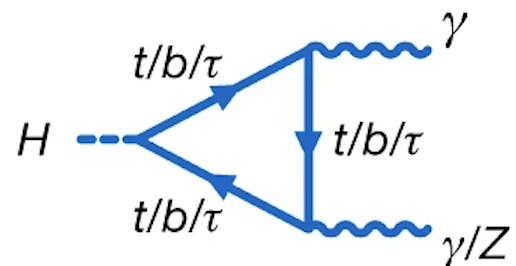
\includegraphics[width=0.3\linewidth]{images/Hgg_loop.png}   \\
        (a) & (b) & (c) \\
    \end{tabular}
    \vspace{0.5em} % Espacio entre filas
    % Segunda fila: 2 imágenes centradas bajo las 3 primeras
    \makebox[\textwidth][c]{%
        \begin{tabular}{cc}
            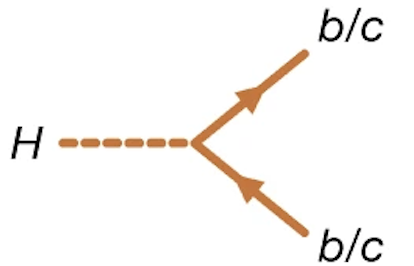
\includegraphics[width=0.3\linewidth]{images/Hbb.png} &
            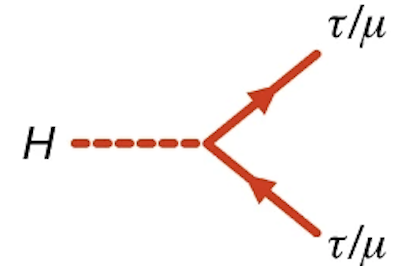
\includegraphics[width=0.3\linewidth]{images/Htt.png} \\
            (d) & (e)  \\
        \end{tabular}%
    }
    \caption{
        Representative LO Feynman diagrams for the main decay modes of a Higgs boson of 125 GeV to (a) a pair of vector bosons, (b) a pair of photons or a $Z$ boson and a photon,
        (c) a pair of quarks, and (d) a pair of charged leptons~\cite{Nature_ATLAS}.}
    \label{fig:h_decays}
\end{figure}


The Higgs boson predominantly decays into a pair of bottom quarks, \( H \rightarrow b\bar{b} \), with a branching ratio of approximately \( \mathcal{B}(H \rightarrow b\bar{b}) \approx 0.581 \). However, the measurement of this decay mode at the \acrshort{lhc} is particularly challenging due to the overwhelming background from multijet production. Despite this, its large branching ratio motivates dedicated studies, especially in channels involving the associated production of a Higgs boson with a vector boson, which enhances sensitivity.

Decays into pairs of gauge bosons are suppressed, since at least one of the two bosons must be produced off-shell due to the limited mass of the Higgs boson. The corresponding branching ratios are approximately \( \mathcal{B}(H \rightarrow WW^*) \approx 0.22 \) and \( \mathcal{B}(H \rightarrow ZZ^*) \approx 0.03 \). Among these, the \( H \rightarrow ZZ^* \) decay mode stands out due to its clean experimental signature and high resolution, as the $Z$ bosons can decay fully leptonically into pairs of electrons or muons that can be efficiently reconstructed and identified in the detector. 
In contrast, for \( H \rightarrow WW^* \), the $W$ bosons can decay hadronically, leading to final states that are more difficult to discriminate from the large \acrshort{qcd} background present in hadron colliders like the \acrshort{lhc}. Alternatively, they can decay leptonically, resulting in final states with neutrinos that escape detection and complicate the event reconstruction.

The Higgs boson can also decay into a pair of photons, \( H \rightarrow \gamma\gamma \), via a one-loop radiative process involving virtual top-antitop quarks or $W$ boson loops. Although this decay has one of the lowest branching ratios, alongside \( H \rightarrow Z\gamma \), with \( \mathcal{B}(H \rightarrow \gamma\gamma) \approx 0.227\% \) and \( \mathcal{B}(H \rightarrow Z\gamma) \approx 0.15\% \), it plays a key role in Higgs boson studies at the \acrshort{lhc} due to its excellent signal-to-background ratio. This leads to a very clean experimental signature with high resolution, especially when compared to the background from prompt photon pair production.

The decay into a pair of $\tau$ leptons is also possible for the \acrshort{sm} Higgs boson, with a branching ratio of approximately 6\%. This decay mode plays a central role in this thesis. From the experimental point of view, the $H \rightarrow \tau\tau$ decay presents several challenges. Firstly, the presence of neutrinos in tau decays prevents a full reconstruction of the di-tau final state, complicating the determination of the Higgs boson mass. To overcome this limitation, advanced reconstruction techniques must be employed to estimate the mass of the di-$\tau$ system.

Secondly, the $H \rightarrow \tau\tau$ decay is affected by a significant background from $Z \rightarrow \tau\tau$ events, whose production cross-section is several orders of magnitude larger than that of the Higgs boson. Despite these difficulties, this decay channel offers an unique opportunity to probe the Yukawa interaction between the Higgs boson and the tau lepton, providing the most precise measurement of a fermionic coupling to date due to its relatively large branching ratio. Furthermore, it allows for the study of the CP properties of the Higgs boson, both in its production mechanisms and decay, and offers good sensitivity to the vector boson fusion (VBF) production mode.

In the context of the Yukawa sector, the \acrshort{sm} also predicts Higgs boson decays to fermions of the first and second generation. The decay into muons, \( H \rightarrow \mu\mu \), although having a very small branching ratio of about 0.02\%, presents a clean experimental signature with two well-reconstructed muons in the final state. However, its measurement is significantly affected by the dominant background from the Drell--Yan process. On the other hand, the \( H \rightarrow c\bar{c} \) decay has a larger branching ratio of approximately 2.9\%, but its measurement at the \acrshort{lhc} is hampered by the large \acrshort{qcd} multijet background. In addition, the identification of charm quarks remains a difficult task in the environment of a hadron collider. Decays of the Higgs boson to lighter fermions have exceedingly small branching fractions, rendering their direct observation unfeasible with current experimental sensitivity~\cite{https://doi.org/10.23731/cyrm-2017-002}.

%xxxxxxxxxxxxxxxxxxxxxxxxxxxxxxxxxxxxxxxxxxxxxxxxxxxxxx
\subsection{The \ttH process: a gateway to the Yukawa sector}
\label{sec:ttH}
%xxxxxxxxxxxxxxxxxxxxxxxxxxxxxxxxxxxxxxxxxxxxxxxxxxxxxx
As already highlighted in previous sections, the top quark Yukawa coupling, $y_t$, is the strongest among all Standard Model fermions, owing to the large mass of the top quark. This makes $y_t$ particularly sensitive to possible \acrshort{bsm} contributions and an essential parameter to explore the nature of electroweak symmetry breaking~\cite{Englert:2014uua,Dobrescu:1997nm,Chivukula:1998wd,Delepine:1995qs}. Moreover, direct access to $y_t$ is crucial for probing the CP structure of the Higgs sector~\cite{Bernreuther:2002uj,Brod:2013cka}, and plays an indirect role in constraining the Higgs self-coupling~\cite{Buttazzo:2013uya,Degrassi:2016wml}.

While a direct measurement via the $H\to t\bar{t}$ decay is not accessible due to kinematic suppression because of top quarks large mass, the associated production of a Higgs boson with a top-quark pair $t\bar{t}H$ offers an unique and direct probe of $y_t$. Contrary to (\acrshort{ggf}), where the coupling appears in a loop and may receive \acrshort{bsm} contributions, the \ttH process provides tree-level sensitivity to $y_t$. This complementarity is particularly useful when comparing indirect constraints from loop-induced processes to direct measurements~\cite{Ng:1983jm,Kunszt:1984ri,Beenakker:2001rj}.

The \ttH production mode was first observed in 2018 by the ATLAS and CMS collaborations~\cite{ATLAS:2018mme,CMS:2018uxb}, following the combination of multiple analyses targeting different Higgs boson decay channels. Among these, the $H\to b \bar{b}$ and $H\to \gamma \gamma$ analyses provided the first observations due to their high branching ratio or clean experimental signature, respectively. However, both channels come with significant limitations: the former suffers from large backgrounds with additional $b$-jets and sizeable modeling uncertainties, while the latter is constrained by its very low branching fraction.

The decay of the Higgs boson to a pair of $\tau$ leptons offers an alternative approach that strikes a balance between statistical power and experimental cleanliness. The $H\to\tau\tau$ branching ratio is significantly larger than that of $H\to \gamma \gamma$, and although $\tau$ leptons are more challenging to reconstruct than electrons or muons, they produce relatively clean final states. Furthermore, $H\to\tau\tau$ decays provide unique sensitivity to the Yukawa coupling to leptons and to potential CP-violating effects in the Higgs sector.

The analysis of \ttH production with $H\to\tau\tau$ decays is typically grouped with other multilepton ($H\to WW^*, ZZ^*$) final states, due to similarities in event topology. This grouping facilitates background suppression and signal extraction strategies, though it makes the isolation of the di-$\tau$ system contribution more challenging. 

However, the main analysis presented in this thesis focuses on the case where both $\tau$ leptons decay hadronically. This channel is not included within the leptonic or semileptonic categories of the $t\bar{t}H \to \tau\tau$ analyses, which are integrated into the aforementioned ``multilepton analysis''. Instead, it is treated as part of the $H\to\tau\tau$ analysis, which will be introduced later and combines $t\bar{t}H$ with other production modes, in semileptonic, dileptonic, and fully hadronic final states. In Section~\ref{analysis}, it will be exploited the distinctive experimental signature and the potential of this process.



%xxxxxxxxxxxxxxxxxxxxxxxxxxxxxxxxxxxxxxxxxxxxxxxxxxxxxx
\subsection{Measurements of cross-section and branching ratios: the STXS framework}
\label{sec:stxs_yukawa}
%xxxxxxxxxxxxxxxxxxxxxxxxxxxxxxxxxxxxxxxxxxxxxxxxxxxxxx


Measurements targeting a Higgs boson signal commonly focus on determining a signal strength modifier, denoted as $\mu$. This parameter is defined as the ratio of the measured production cross-section times the branching ratio to the corresponding Standard Model (\acrshort{sm}) prediction, i.e.,
\begin{equation}
\label{signal_strength}
    \mu = \frac{\sigma \times \mathcal{B}}{\sigma_{\mathrm{\acrshort{sm}}} \times \mathcal{B}_{\mathrm{\acrshort{sm}}}},
\end{equation}
Such measurements aim to maximize sensitivity to the Higgs boson signal by comparing observed event yields in data to the expected yields from the \acrshort{sm} for each of the main Higgs boson production modes.

During the Run 2 period of the Large Hadron Collider (\acrshort{lhc}), all the main Higgs boson production and decay modes have been observed with varying degrees of significance. The latest combined results from the ATLAS experiment for production cross-section and decay branching ratio measurements show a remarkable agreement with \acrshort{sm} expectations, as illustrated in Figure~\ref{higgs_mu}, resulting in a measured inclusive signal strength of $\mu = 1.05 \pm 0.06$~\cite{Nature_ATLAS}. Similar value was obtained by the CMS collaboration~\cite{CMS:2022dwd}. Evidence for rare decay modes, such as $H \to Z\gamma$ and $H \to \mu\mu$, has also been reported~\cite{Aad_2024,muon2021}.

\begin{figure}[htbp]
    \centering
    \begin{tabular}{cc}
    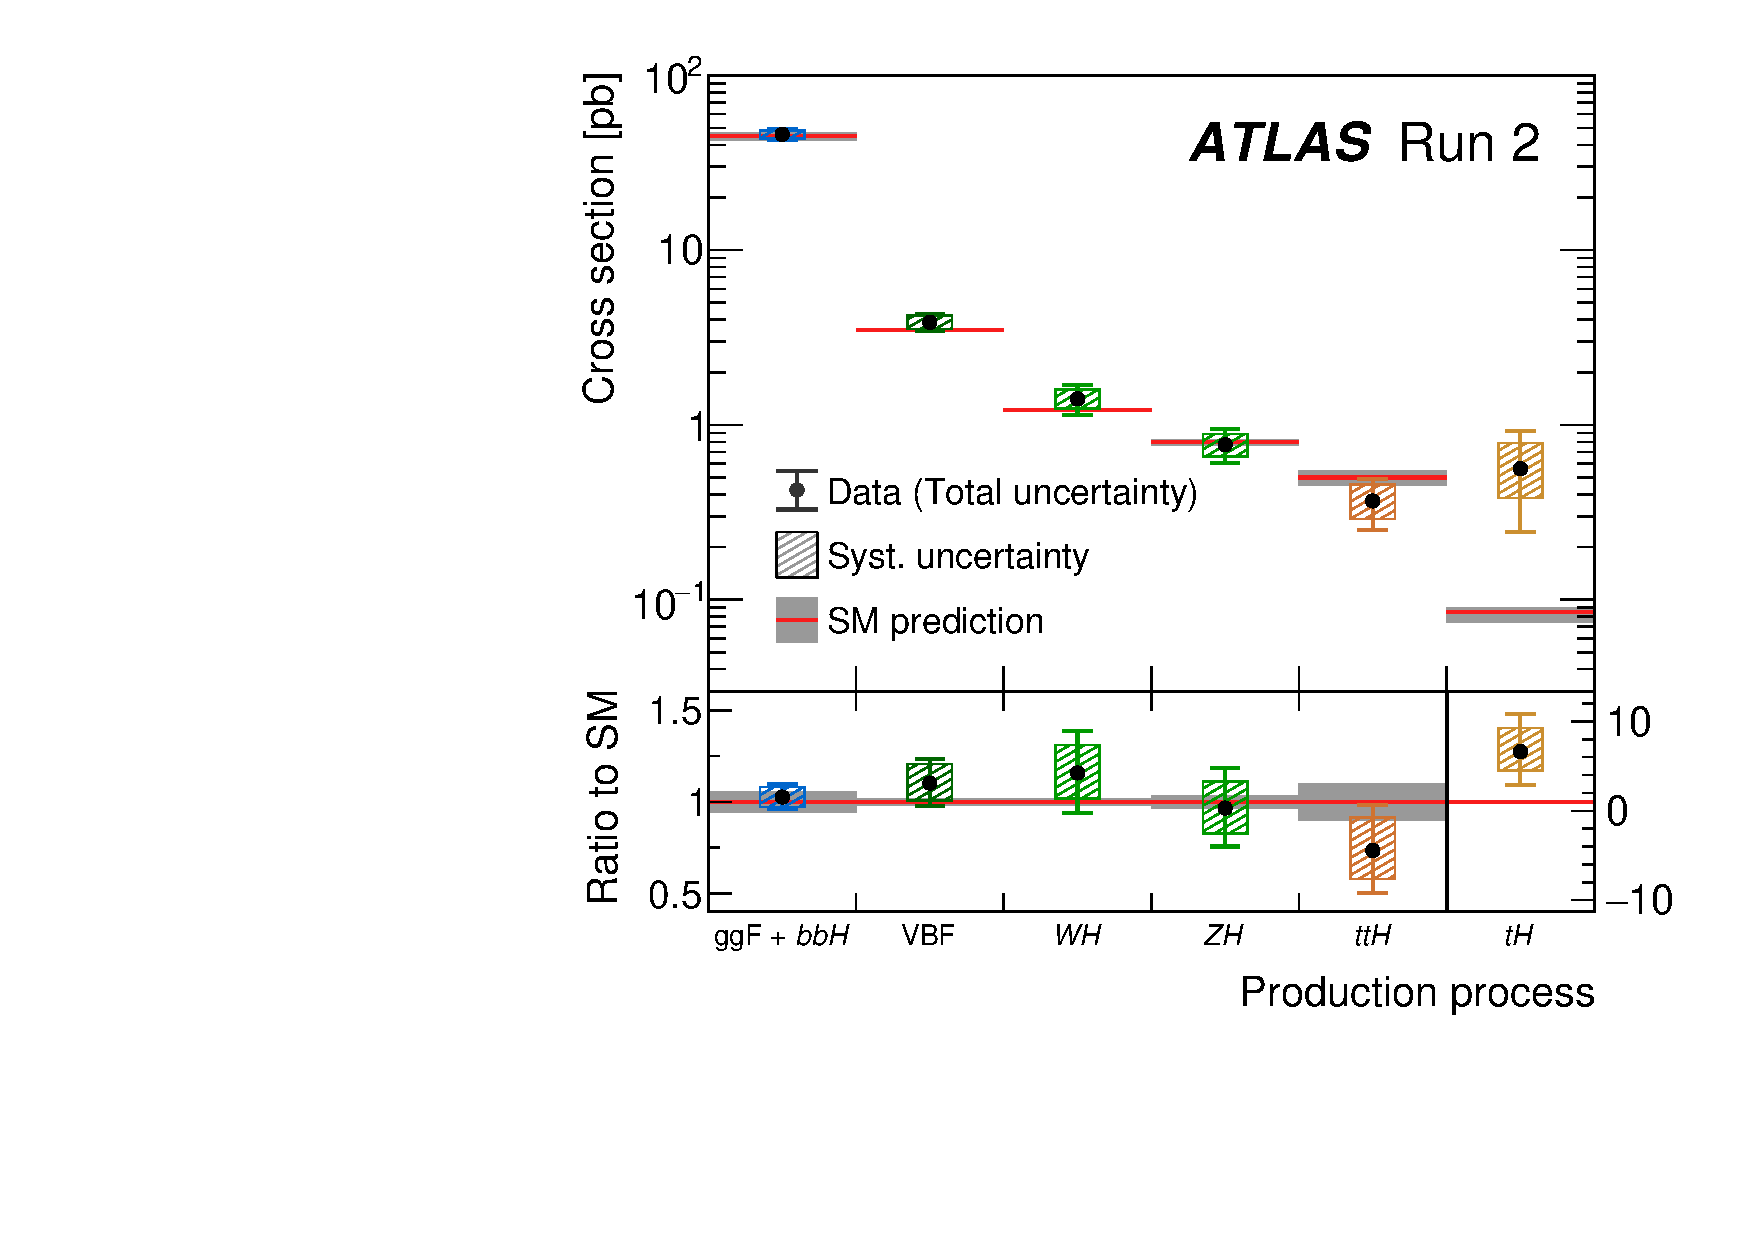
\includegraphics[width=0.46\textwidth]{atlas_combined_xsect.pdf} & 
    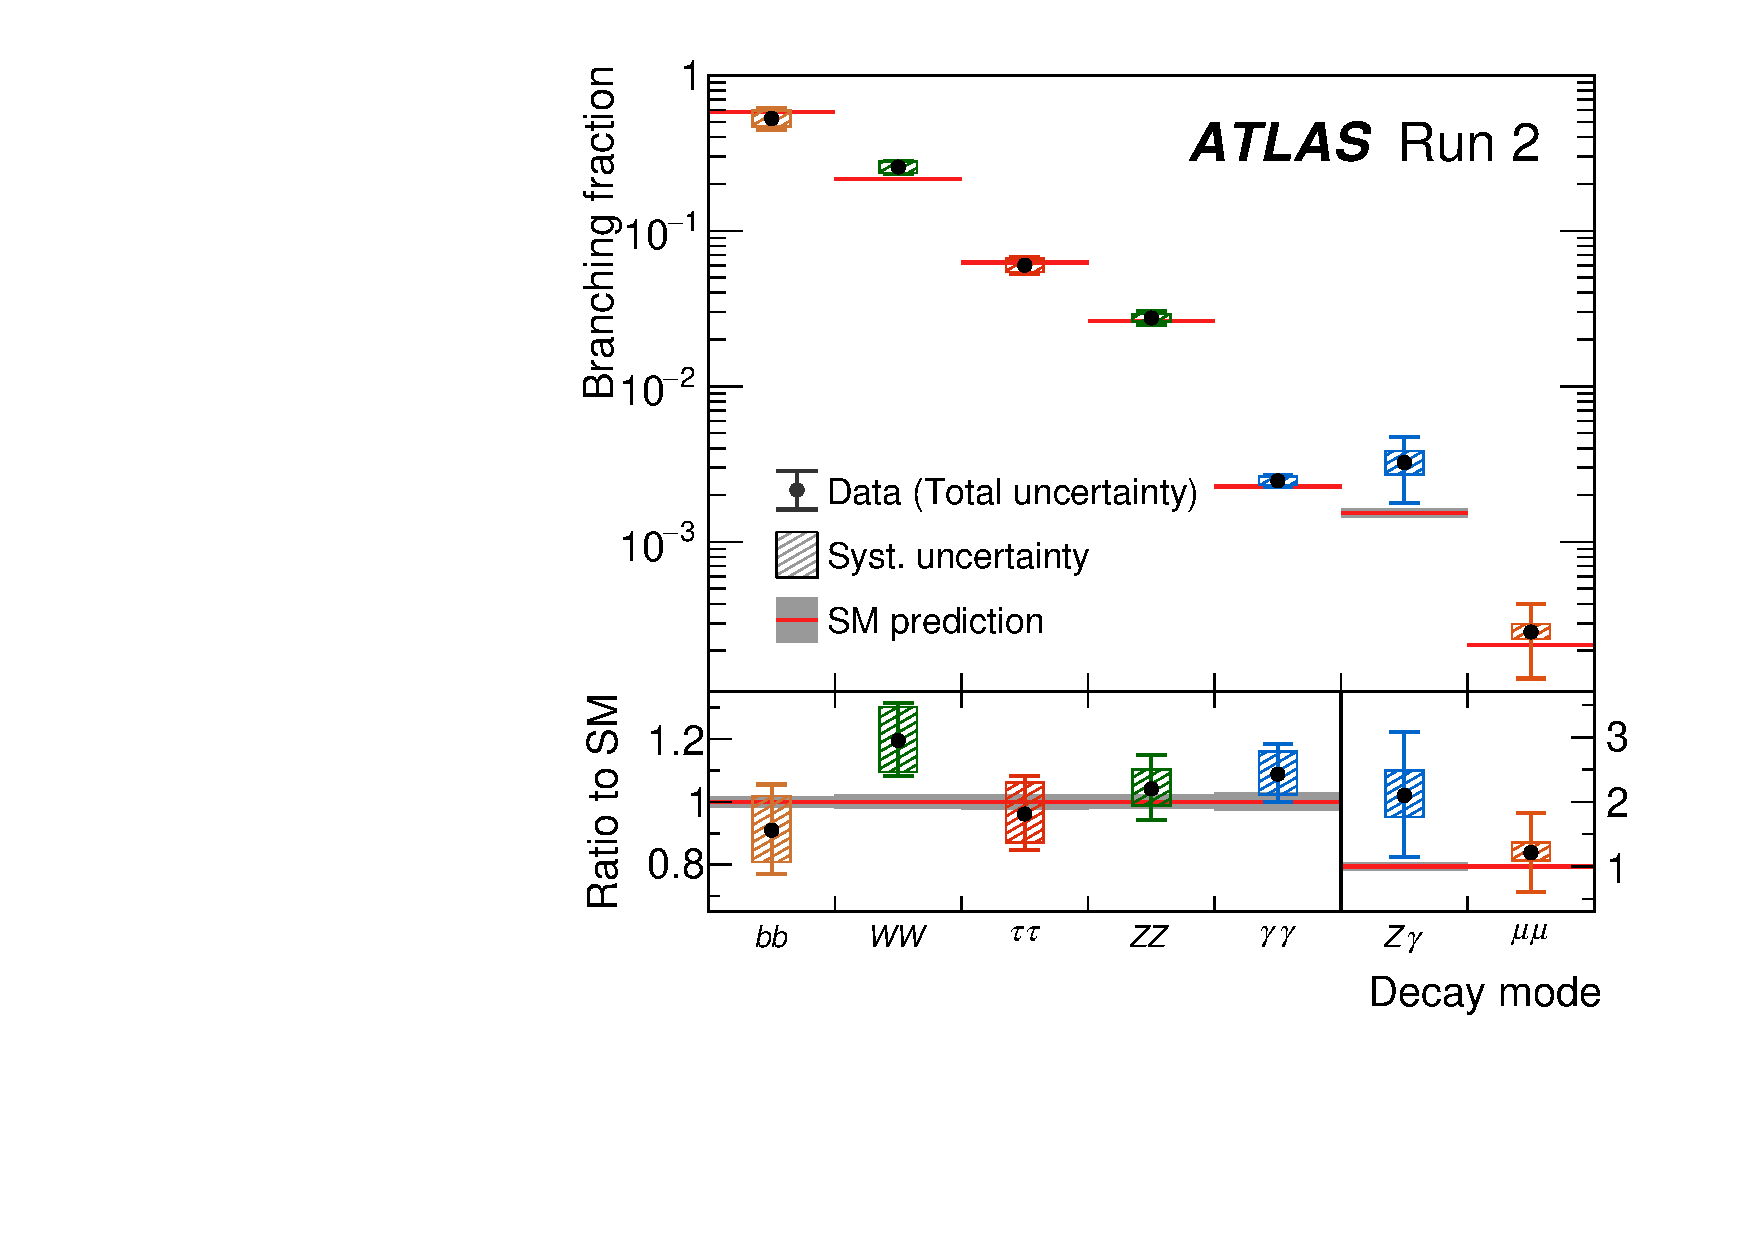
\includegraphics[width=0.46\textwidth]{atlas_combined_br.pdf}
    \end{tabular}
    \caption{Summary of the Higgs boson production cross-section on the left, asumming \acrshort{sm} values for the Higgs boson branching ratios, and decay branching ratio measurements on the right asumming \acrshort{sm} predictions for the production cross-sections. All results were obtained using ATLAS Run 2 data, combining different analysis and are consistent with the \acrshort{sm} predictions within uncertainties~\cite{Nature_ATLAS}.}
    \label{higgs_mu}
\end{figure}

Despite their overall success, these inclusive measurements exhibit limited sensitivity to B\acrshort{sm} effects that could manifest in specific phase space regions where few signal events are expected. Furthermore, these inclusive analyses depend heavily on theoretical predictions, as the uncertainty in the global signal strength $\mu$ is directly influenced by the uncertainties in the \acrshort{sm} cross-section and branching ratio calculations that are assumed. Additionally, analysis strategies and event selection criteria typically assume \acrshort{sm} kinematics for the expected signal, which may reduce sensitivity to B\acrshort{sm} scenarios.

An alternative approach to reduce the dependence on \acrshort{sm} theoretical extrapolations is the measurement of fiducial cross-sections. In these analyses, a fiducial phase space is defined at particle level\footnote{The particle level indicates the level in which all the physical objects are defined using stable particles in their final states, after parton shower and hadronisation, but without any interaction with the detector.}, designed to closely resemble the reconstructed event selections to minimize the extrapolation from the measured phase space. Detector effects are corrected via simulation, allowing a direct comparison of the measured fiducial cross-section with theoretical predictions. However, the requirement of similar selections at particle and detector levels often necessitates simplified event selections, which might not be optimal for signal-to-background discrimination. The use of multivariate techniques is typically limited in fiducial measurements due to the complexity of mapping reconstructed variables to particle-level definitions.

Fiducial cross-section measurements can be further extended to differential cross-section measurements, where the production rates are measured as functions of relevant kinematic observables. These measurements provide richer information on the Higgs boson production dynamics and possible deviations from \acrshort{sm} predictions.

To find a balance between inclusive and fiducial differential measurements, the Simplified Template Cross-Section (STXS) framework has been developed~\cite{badger2016leshouches2015physics}. The STXS framework partitions the Higgs boson production phase space into multiple exclusive regions or bins, each defined by kinematic criteria involving the Higgs boson and associated objects in the final states such as jets or vector bosons. This binning scheme is optimized to enhance sensitivity to possible B\acrshort{sm} effects while keeping a reasonable independence and control over theoretical uncertainties.

STXS measurements offer differential information about Higgs boson production, allowing the use of complex multivariate analysis techniques in event selections. This is particularly advantageous for decay channels with challenging final-state reconstruction, such as $H \to \tau\tau$ or $H \to b\bar{b}$, where detector resolution and background contamination are more significant compared to cleaner channels like $H \to \gamma\gamma$ or $H \to ZZ^*$.

The STXS framework also facilitates the combination of results from analyses targeting different Higgs boson decay modes, maximizing the overall experimental sensitivity. The current binning scheme, referred to as Stage 1.2 and shown in Figure~\ref{fig:STXSbins}, refines the granularity introduced in earlier stages (so called Stage 1.1~\cite{STXS11}) to better exploit the available data. A simplified fiducial volume common to all STXS analyses requires the Higgs boson to have rapidity $|y| < 2.5$, matching the typical detector acceptance, where the pseudorapidity is defined as $y = 0.5 \ln{\left( \frac{E+p_Z}{E-p_Z} \right)}$.

\begin{figure}[htbp]
    \centering
    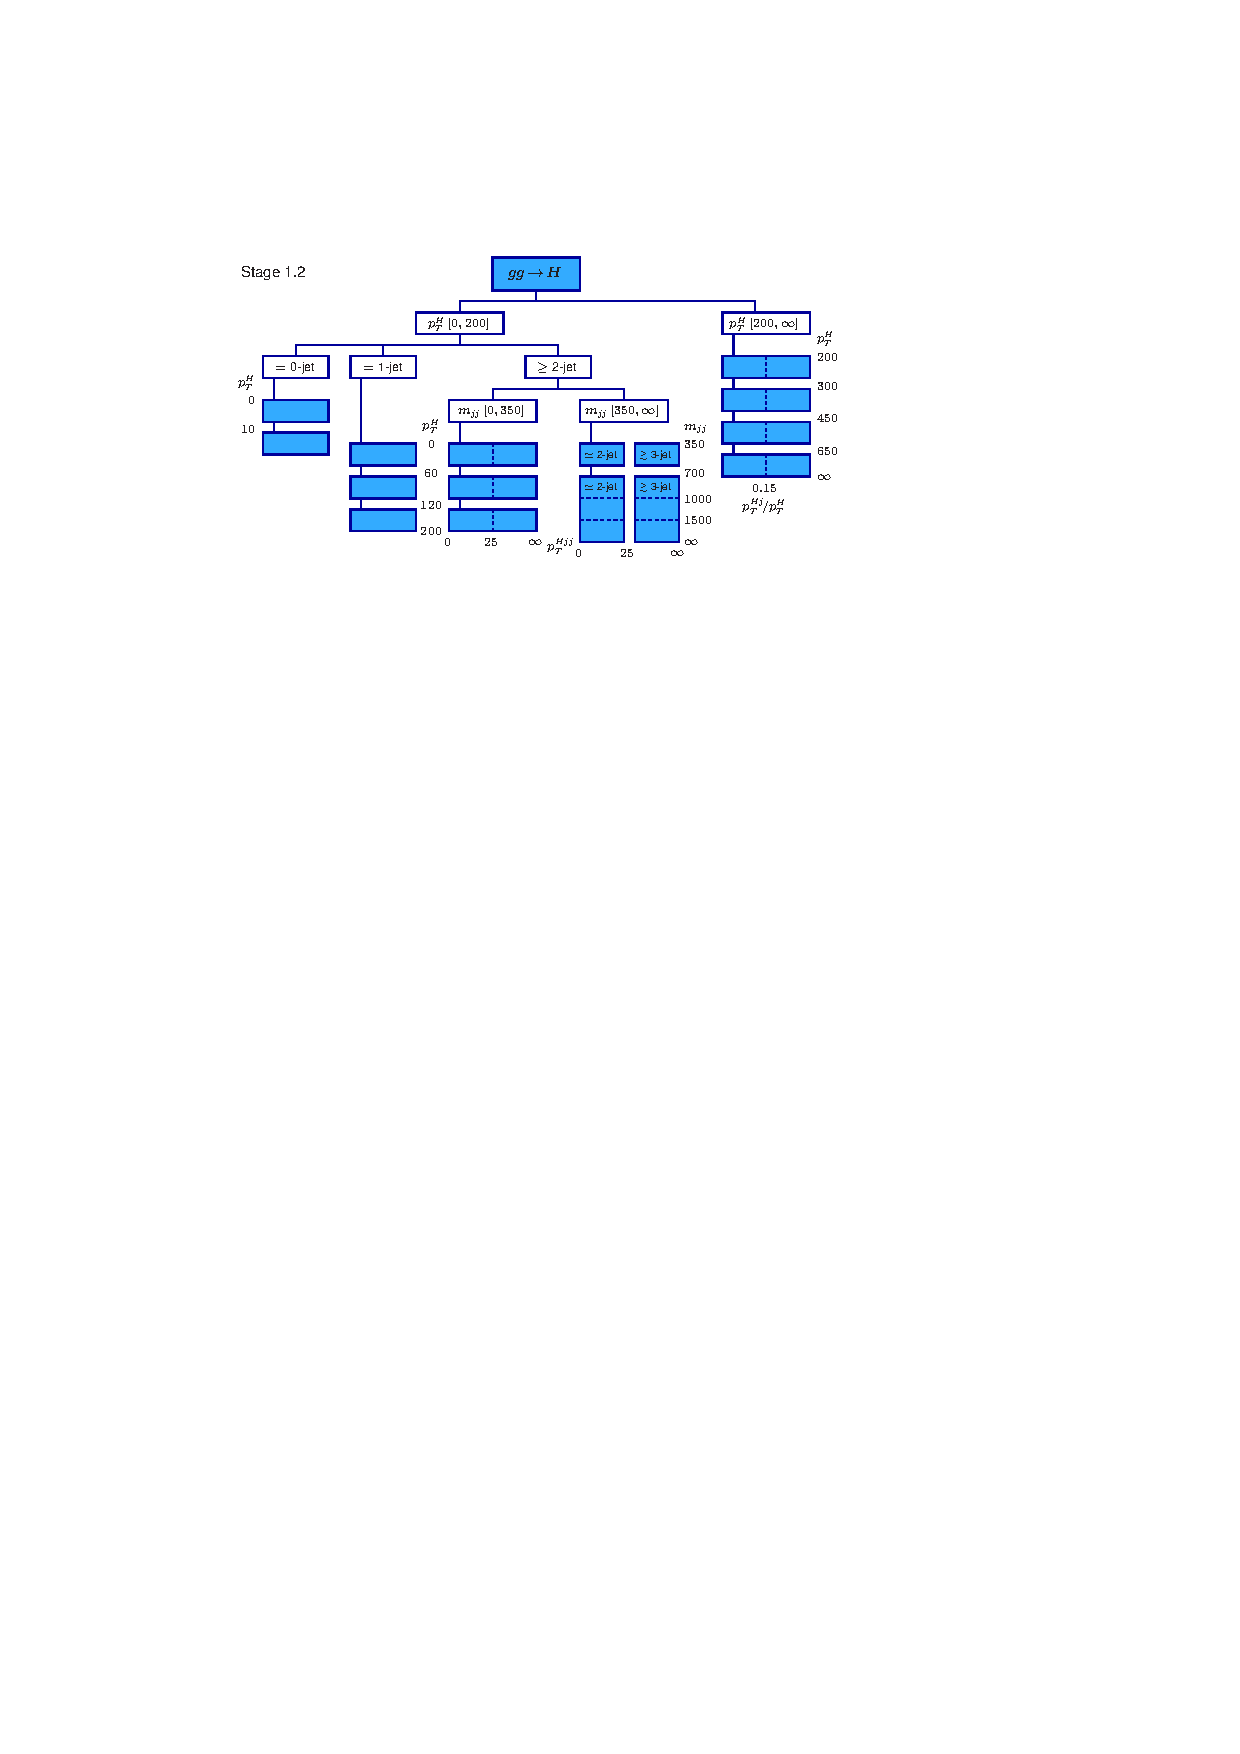
\includegraphics[width=0.6\linewidth]{images/STXSbins_ggF}\\
    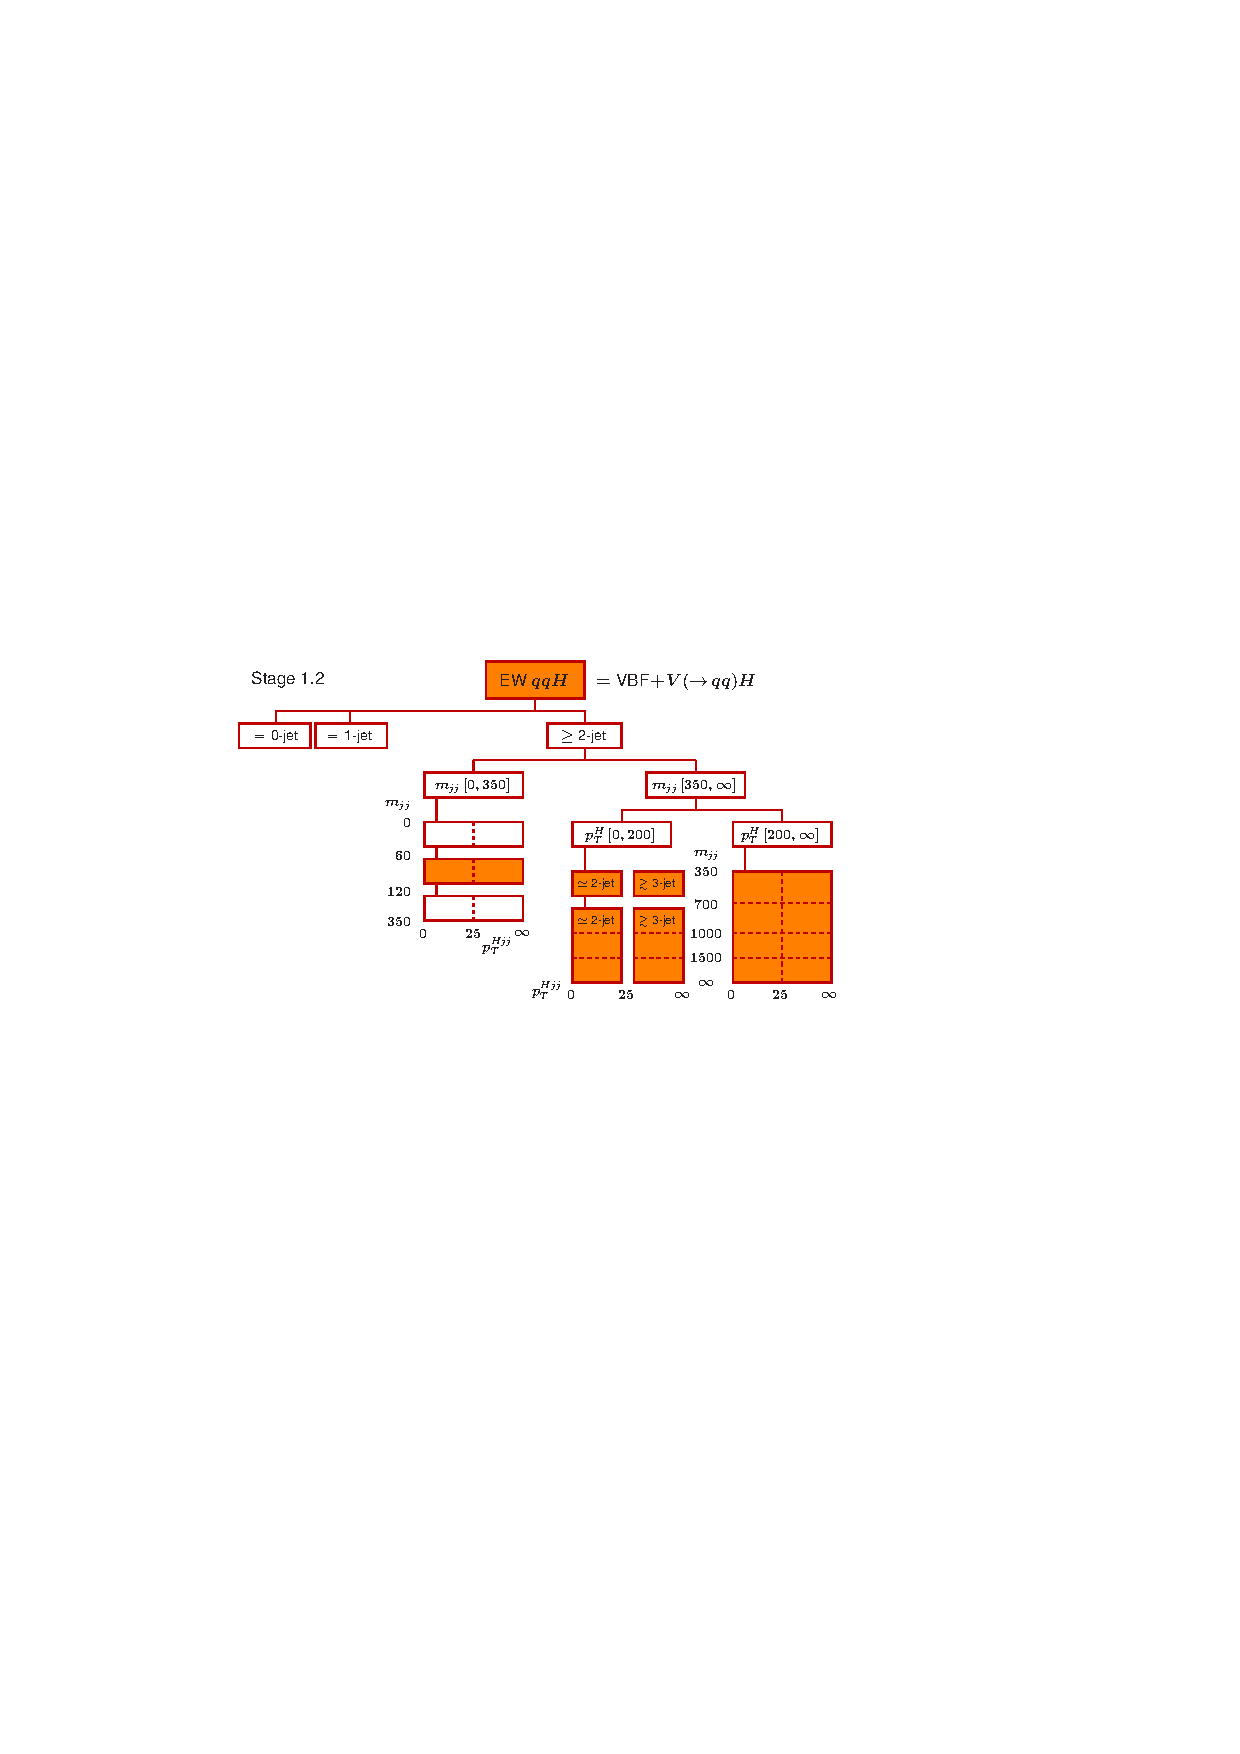
\includegraphics[width=0.6\linewidth]{images/STXSbins_VBF_VqqH}\\
    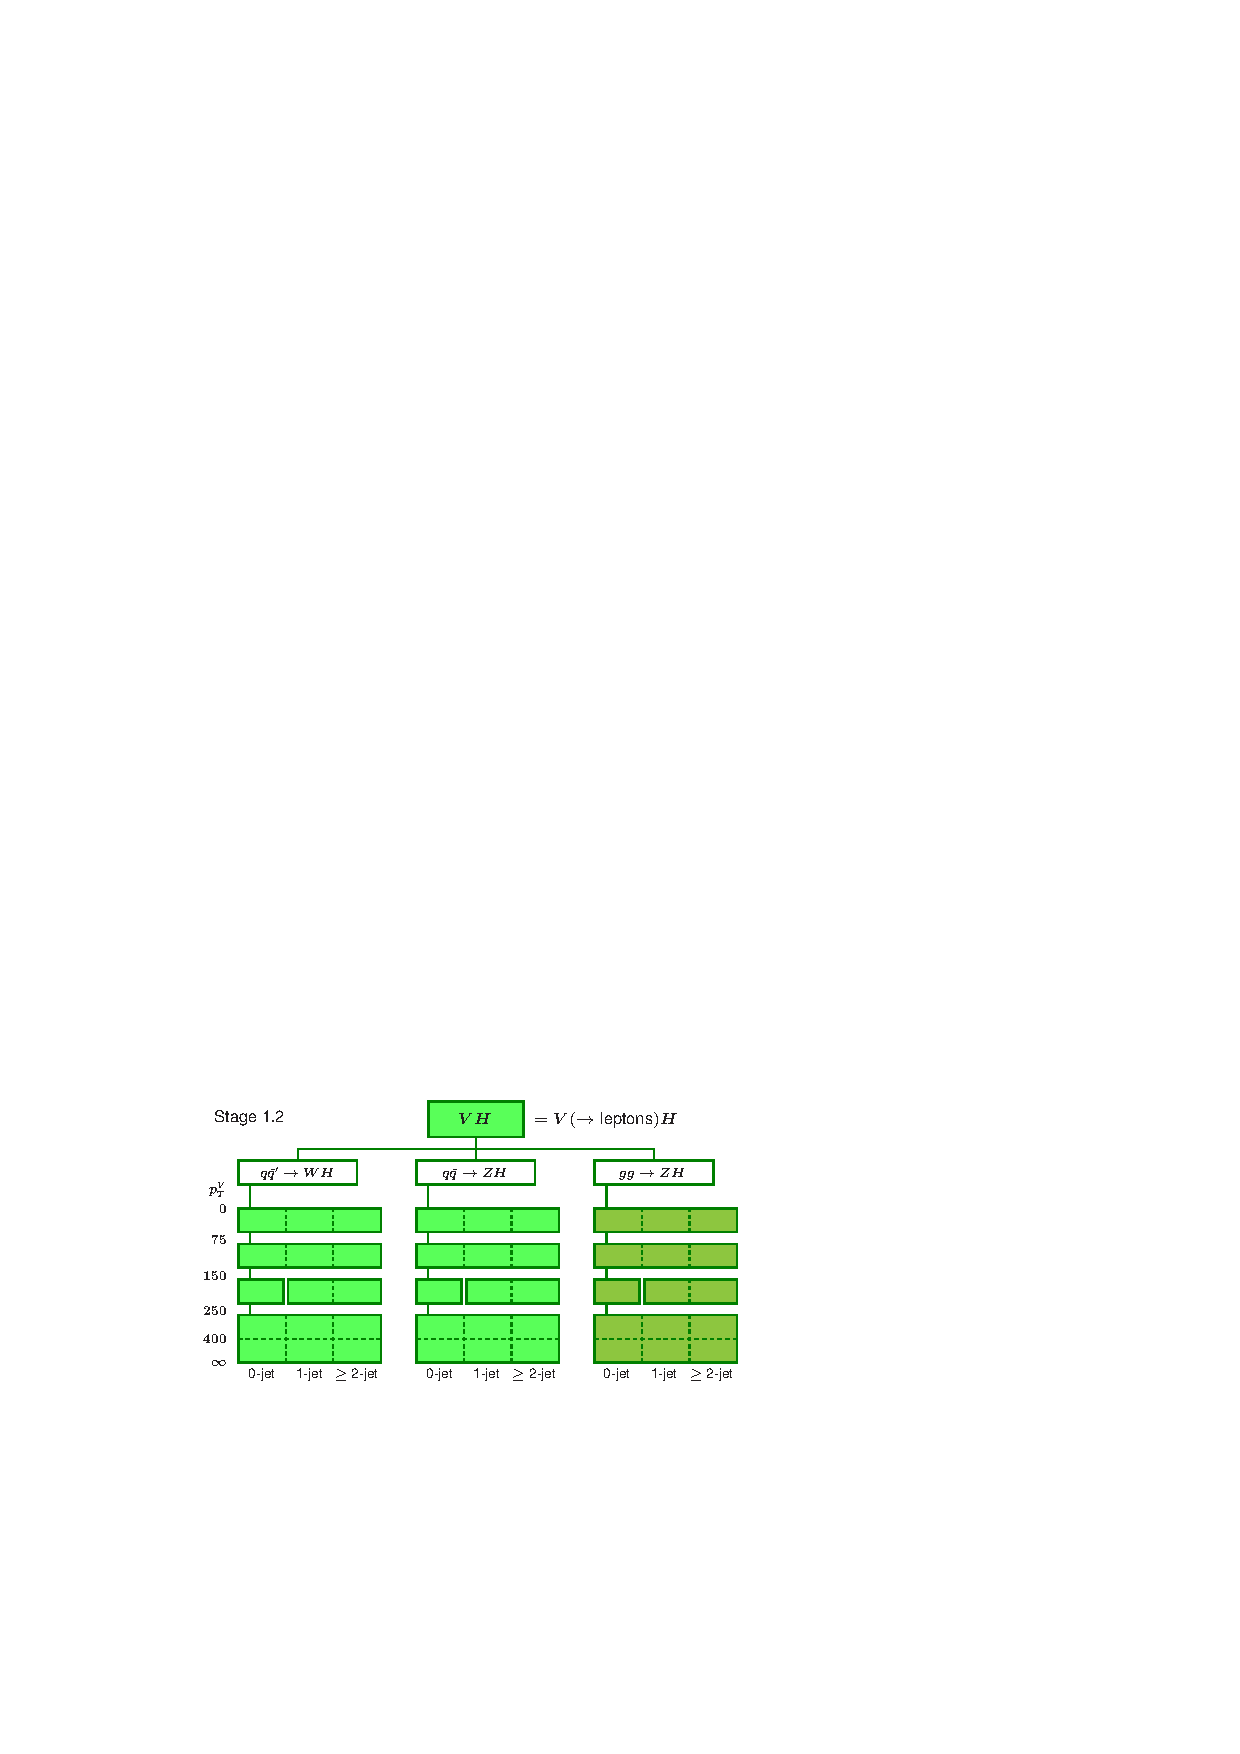
\includegraphics[width=0.6\linewidth]{images/STXSbins_VlepH}\\
    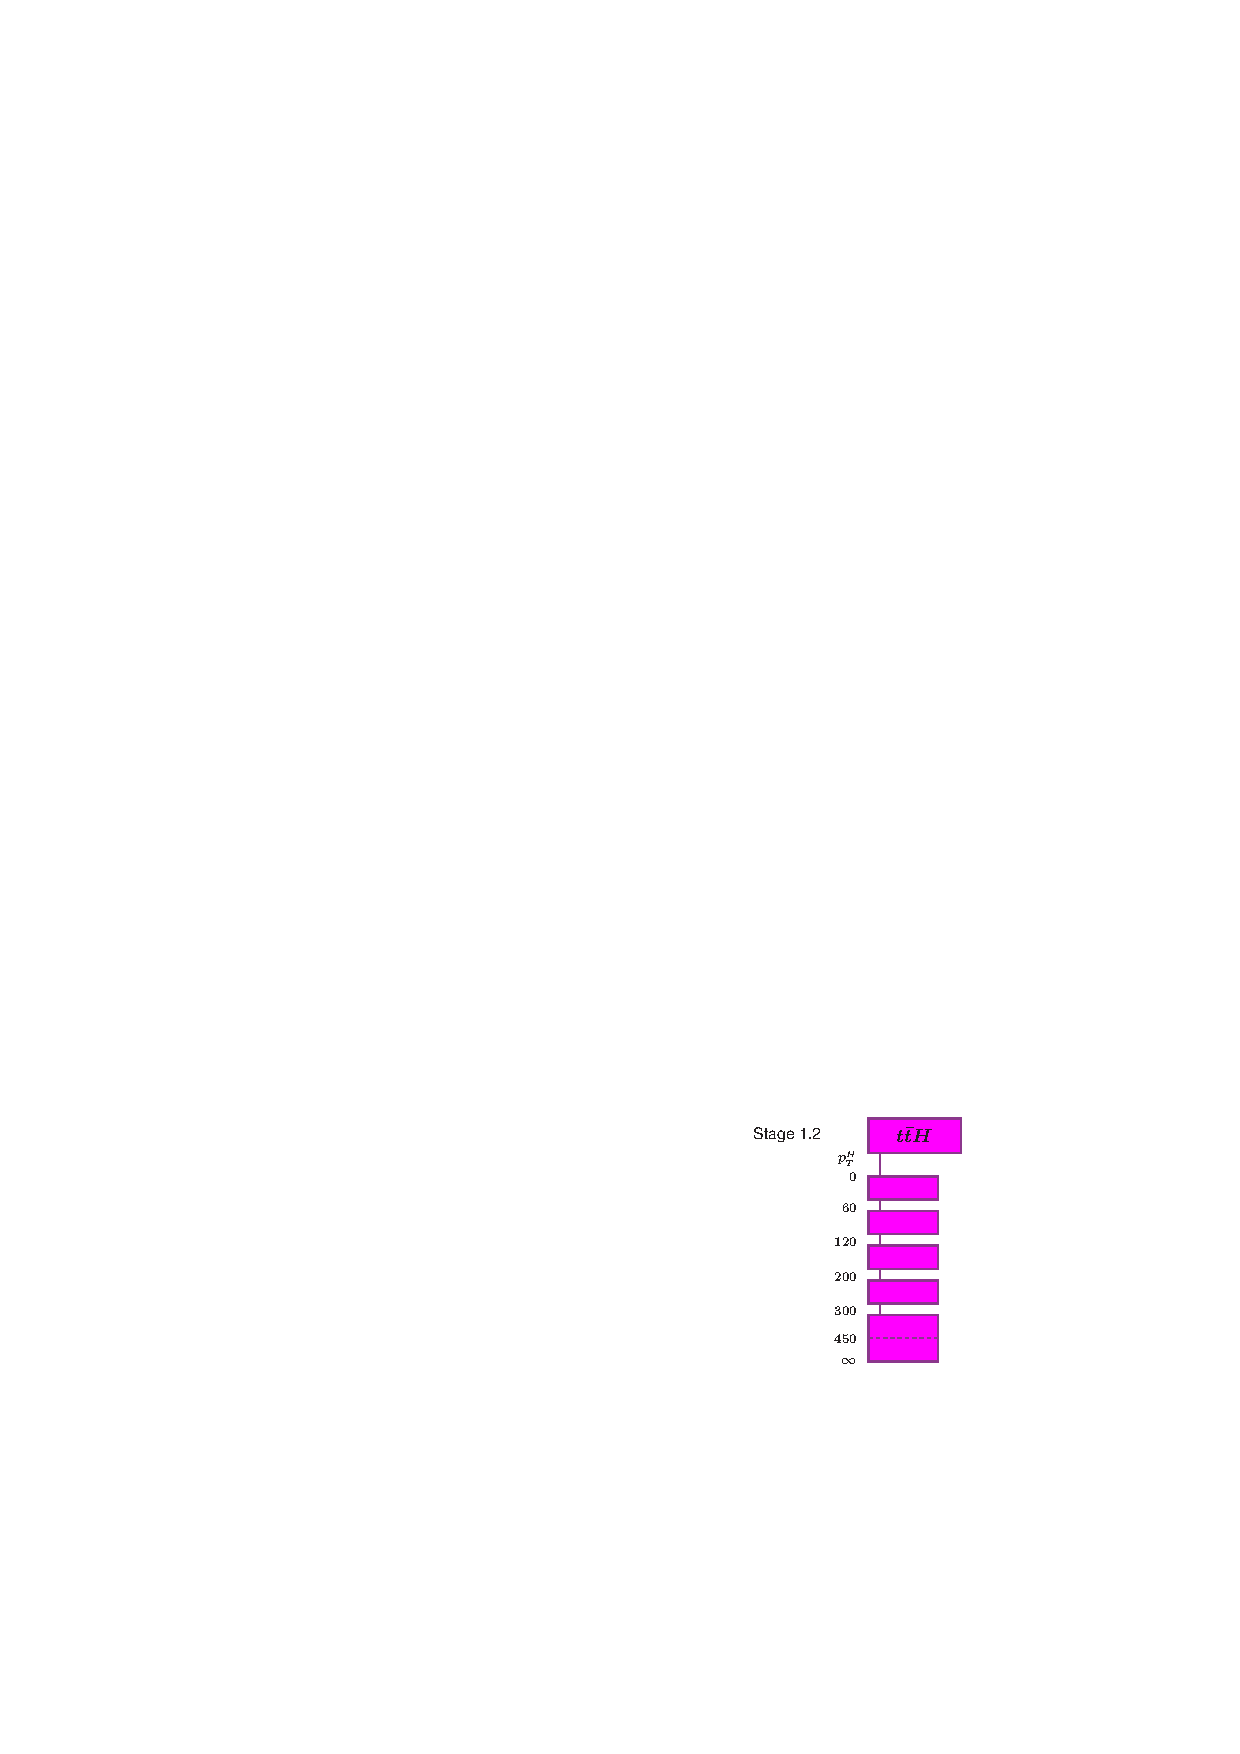
\includegraphics[width=0.25\linewidth]{images/STXSbins_ttH}\\
    \caption{STXS stage 1.2 bin definition for (a) gluon-gluon fusion production, (b) vector boson fusion production and associated production with a hadronically decaying vector boson, (c) associated production with a leptonically-decaying vector boson and (d) associated production with a top-antitop quark pair~\cite{badger2016leshouches2015physics}.}
    \label{fig:STXSbins}
\end{figure}


Higgs boson production modes are classified into categories within the STXS scheme, based on the production mechanism and associated particles:

\begin{itemize}
    \item \textbf{Gluon-gluon fusion (ggF)}: including the dominant gluon-gluon fusion process and gluon-induced associated production with a $Z$ boson decaying hadronically, $gg \to ZH \to q\bar{q}H$. Production of $b\bar{b}H$ is also included here.
    \item \textbf{$qq'\to qq'H$}: it includes the Higgs boson production via fusion of vector bosons and quark-initiated associated production of a Higgs boson with a vector boson where the vector boson decays hadronically ($qq'\to VH \to qq'H$).
    \item \textbf{Vector boson associated production ($VH \to (ll, l\nu)H$)}: Higgs boson produced in association with a $W$ or $Z$ boson decaying leptonically.
    \item \textbf{Top-associated production ($t\bar{t}H$ and $tH$)}: Higgs boson produced with a top quark pair or single top quark (in a single bin).
\end{itemize}

Within each category, the STXS bins are further subdivided based on key variables such as the transverse momentum of the Higgs boson ($p^H_T$) or vector boson ($p^V_T$), the number of jets, and the invariant mass of leading jets. The binning scheme is flexible and can be adapted to the experimental sensitivity: bins with insufficient data can be merged, and finer bins can be introduced as more data becomes available.

The latest combination of ATLAS Run 2 data using the STXS framework has produced measurements of the Higgs boson production cross-section in 36 exclusive kinematic regions~\cite{Nature_ATLAS}. The results are consistent with \acrshort{sm} predictions, providing stringent constraints on \acrshort{bsm} scenarios. Figure~\ref{fig:atlas-stxs-results} summarizes these measurements.

\begin{figure}[htbp]
    \centering
    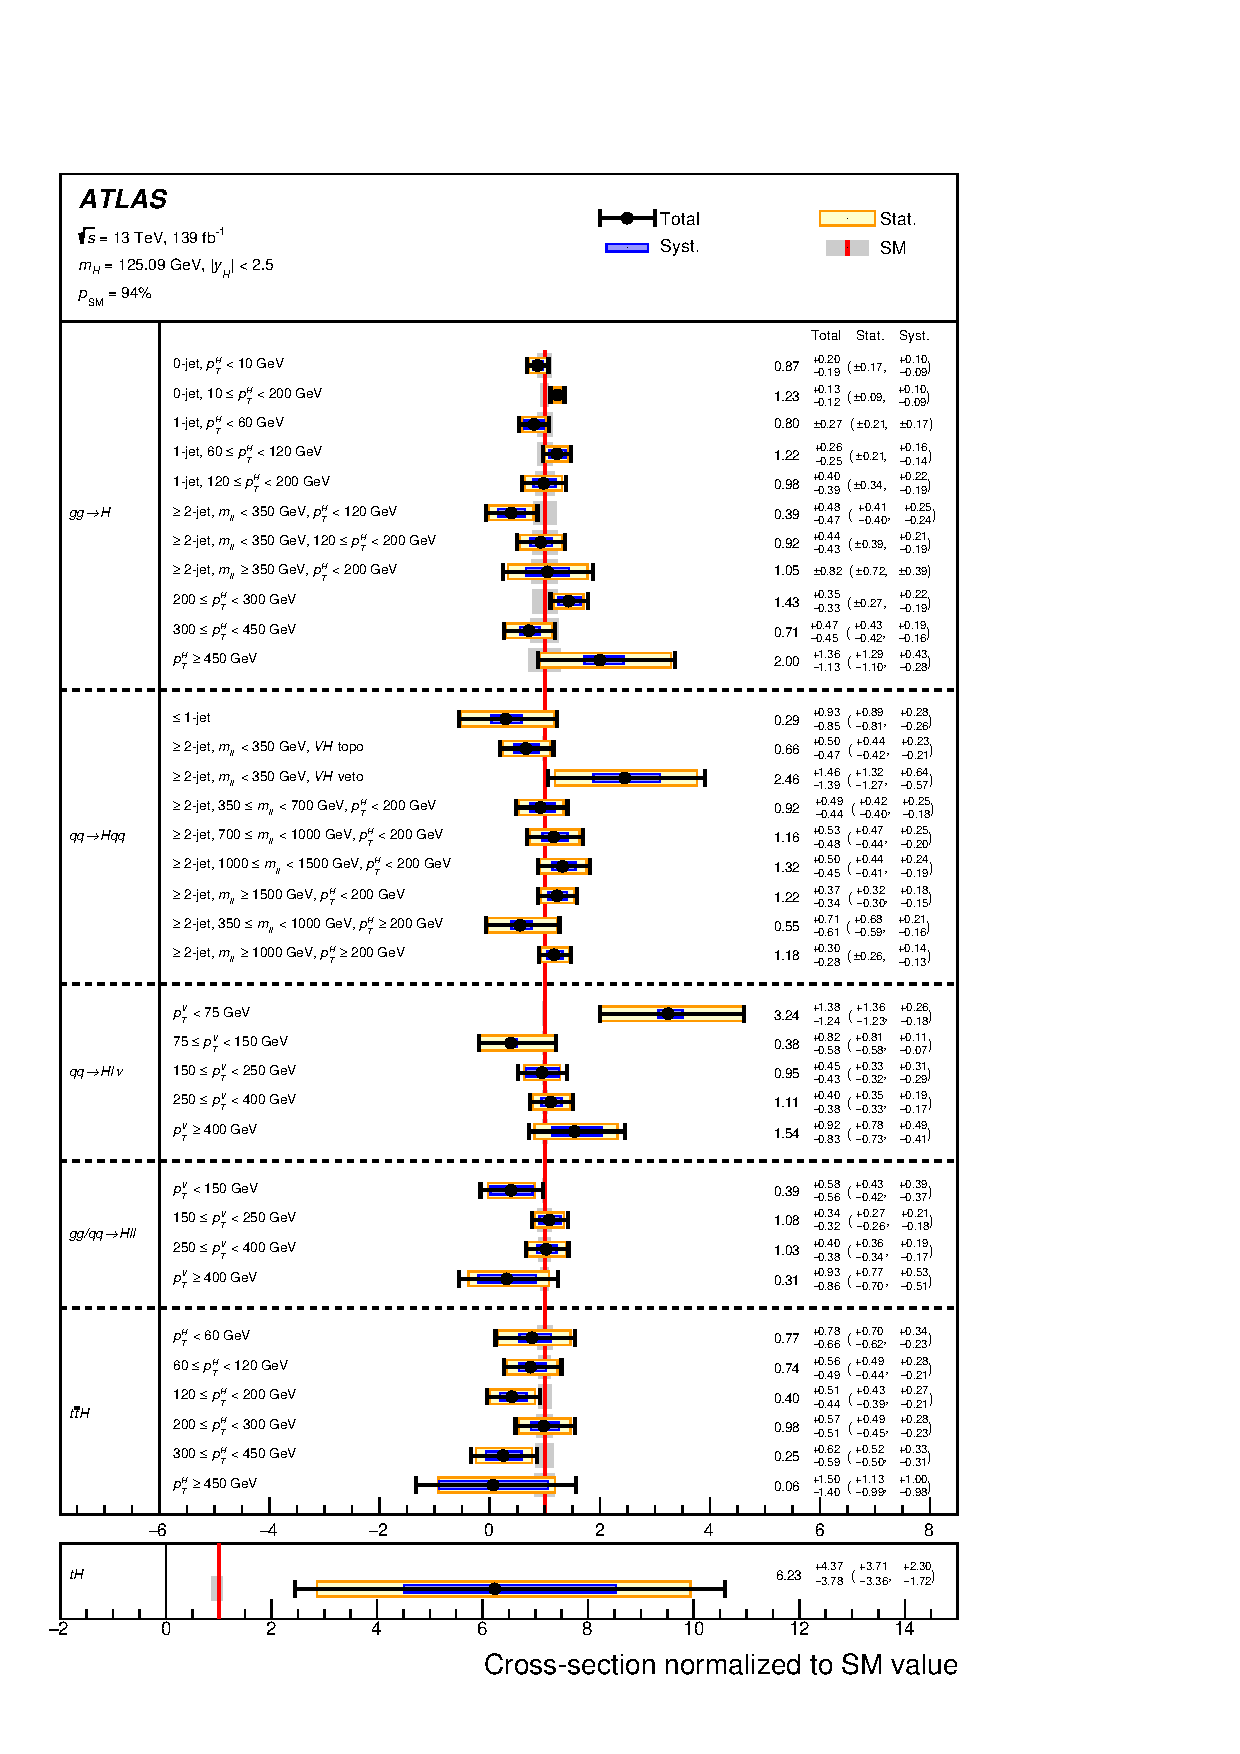
\includegraphics[width=0.75\textwidth]{atlas_stxs_results.pdf}
    \caption{Measurement of the Higgs boson production cross-section normalized to the \acrshort{sm} predictions in 36 exclusive STXS regions using ATLAS Run 2 data. All these results are obtained assuming \acrshort{sm} branching ratios for the Higgs boson decays. The error bars represent the total uncertainty in the measurement (in black), the statistical uncertainty (in yellow) and the systematic uncertainty (in blue)~\cite{Nature_ATLAS}.}
    \label{fig:atlas-stxs-results}
\end{figure}

This thesis contributes to extending the STXS measurements in the $H \to \tau \tau$ decay channel, with particular emphasis on the $t\bar{t}H$ production mode. The analysis strategy and detailed results are presented in Chapter~\ref{analysis}. Note that the results shown in Figure~\ref{fig:atlas-stxs-results} do not yet include the $H \to \tau \tau$ channel measurements presented in this document.

